\documentclass[ignorenonframetext,]{beamer}
\setbeamertemplate{caption}[numbered]
\setbeamertemplate{caption label separator}{: }
\setbeamercolor{caption name}{fg=normal text.fg}
\beamertemplatenavigationsymbolsempty
\usepackage{lmodern}
\usepackage{amssymb,amsmath}
\usepackage{ifxetex,ifluatex}
\usepackage{fixltx2e} % provides \textsubscript
\ifnum 0\ifxetex 1\fi\ifluatex 1\fi=0 % if pdftex
\usepackage[T1]{fontenc}
\usepackage[utf8]{inputenc}
\else % if luatex or xelatex
\ifxetex
\usepackage{mathspec}
\else
\usepackage{fontspec}
\fi
\defaultfontfeatures{Ligatures=TeX,Scale=MatchLowercase}
\fi
% use upquote if available, for straight quotes in verbatim environments
\IfFileExists{upquote.sty}{\usepackage{upquote}}{}
% use microtype if available
\IfFileExists{microtype.sty}{%
\usepackage{microtype}
\UseMicrotypeSet[protrusion]{basicmath} % disable protrusion for tt fonts
}{}
\newif\ifbibliography
\usepackage{color}
\usepackage{fancyvrb}
\newcommand{\VerbBar}{|}
\newcommand{\VERB}{\Verb[commandchars=\\\{\}]}
\DefineVerbatimEnvironment{Highlighting}{Verbatim}{commandchars=\\\{\}}
% Add ',fontsize=\small' for more characters per line
\usepackage{framed}
\definecolor{shadecolor}{RGB}{248,248,248}
\newenvironment{Shaded}{\begin{snugshade}}{\end{snugshade}}
\newcommand{\KeywordTok}[1]{\textcolor[rgb]{0.13,0.29,0.53}{\textbf{{#1}}}}
\newcommand{\DataTypeTok}[1]{\textcolor[rgb]{0.13,0.29,0.53}{{#1}}}
\newcommand{\DecValTok}[1]{\textcolor[rgb]{0.00,0.00,0.81}{{#1}}}
\newcommand{\BaseNTok}[1]{\textcolor[rgb]{0.00,0.00,0.81}{{#1}}}
\newcommand{\FloatTok}[1]{\textcolor[rgb]{0.00,0.00,0.81}{{#1}}}
\newcommand{\ConstantTok}[1]{\textcolor[rgb]{0.00,0.00,0.00}{{#1}}}
\newcommand{\CharTok}[1]{\textcolor[rgb]{0.31,0.60,0.02}{{#1}}}
\newcommand{\SpecialCharTok}[1]{\textcolor[rgb]{0.00,0.00,0.00}{{#1}}}
\newcommand{\StringTok}[1]{\textcolor[rgb]{0.31,0.60,0.02}{{#1}}}
\newcommand{\VerbatimStringTok}[1]{\textcolor[rgb]{0.31,0.60,0.02}{{#1}}}
\newcommand{\SpecialStringTok}[1]{\textcolor[rgb]{0.31,0.60,0.02}{{#1}}}
\newcommand{\ImportTok}[1]{{#1}}
\newcommand{\CommentTok}[1]{\textcolor[rgb]{0.56,0.35,0.01}{\textit{{#1}}}}
\newcommand{\DocumentationTok}[1]{\textcolor[rgb]{0.56,0.35,0.01}{\textbf{\textit{{#1}}}}}
\newcommand{\AnnotationTok}[1]{\textcolor[rgb]{0.56,0.35,0.01}{\textbf{\textit{{#1}}}}}
\newcommand{\CommentVarTok}[1]{\textcolor[rgb]{0.56,0.35,0.01}{\textbf{\textit{{#1}}}}}
\newcommand{\OtherTok}[1]{\textcolor[rgb]{0.56,0.35,0.01}{{#1}}}
\newcommand{\FunctionTok}[1]{\textcolor[rgb]{0.00,0.00,0.00}{{#1}}}
\newcommand{\VariableTok}[1]{\textcolor[rgb]{0.00,0.00,0.00}{{#1}}}
\newcommand{\ControlFlowTok}[1]{\textcolor[rgb]{0.13,0.29,0.53}{\textbf{{#1}}}}
\newcommand{\OperatorTok}[1]{\textcolor[rgb]{0.81,0.36,0.00}{\textbf{{#1}}}}
\newcommand{\BuiltInTok}[1]{{#1}}
\newcommand{\ExtensionTok}[1]{{#1}}
\newcommand{\PreprocessorTok}[1]{\textcolor[rgb]{0.56,0.35,0.01}{\textit{{#1}}}}
\newcommand{\AttributeTok}[1]{\textcolor[rgb]{0.77,0.63,0.00}{{#1}}}
\newcommand{\RegionMarkerTok}[1]{{#1}}
\newcommand{\InformationTok}[1]{\textcolor[rgb]{0.56,0.35,0.01}{\textbf{\textit{{#1}}}}}
\newcommand{\WarningTok}[1]{\textcolor[rgb]{0.56,0.35,0.01}{\textbf{\textit{{#1}}}}}
\newcommand{\AlertTok}[1]{\textcolor[rgb]{0.94,0.16,0.16}{{#1}}}
\newcommand{\ErrorTok}[1]{\textcolor[rgb]{0.64,0.00,0.00}{\textbf{{#1}}}}
\newcommand{\NormalTok}[1]{{#1}}
\usepackage{longtable,booktabs}
\usepackage{caption}
% These lines are needed to make table captions work with longtable:
\makeatletter
\def\fnum@table{\tablename~\thetable}
\makeatother
\usepackage{graphicx,grffile}
\makeatletter
\def\maxwidth{\ifdim\Gin@nat@width>\linewidth\linewidth\else\Gin@nat@width\fi}
\def\maxheight{\ifdim\Gin@nat@height>\textheight0.8\textheight\else\Gin@nat@height\fi}
\makeatother
% Scale images if necessary, so that they will not overflow the page
% margins by default, and it is still possible to overwrite the defaults
% using explicit options in \includegraphics[width, height, ...]{}
\setkeys{Gin}{width=\maxwidth,height=\maxheight,keepaspectratio}

% Prevent slide breaks in the middle of a paragraph:
\widowpenalties 1 10000
\raggedbottom

\AtBeginPart{
\let\insertpartnumber\relax
\let\partname\relax
\frame{\partpage}
}
\AtBeginSection{
\ifbibliography
\else
\let\insertsectionnumber\relax
\let\sectionname\relax
\frame{\sectionpage}
\fi
}
\AtBeginSubsection{
\let\insertsubsectionnumber\relax
\let\subsectionname\relax
\frame{\subsectionpage}
}

\setlength{\parindent}{0pt}
\setlength{\parskip}{6pt plus 2pt minus 1pt}
\setlength{\emergencystretch}{3em}  % prevent overfull lines
\providecommand{\tightlist}{%
\setlength{\itemsep}{0pt}\setlength{\parskip}{0pt}}
\setcounter{secnumdepth}{0}
% \usepackage[table]{xcolor}
\usepackage{array}
\usepackage{lscape}
\newcommand{\blandscape}{\begin{landscape}}
\newcommand{\elandscape}{\end{landscape}}
\usepackage{dcolumn}
\usepackage{bbm}
\usepackage{rotating, graphicx}
\usepackage{tabulary}
\usepackage{multirow}
\usepackage{algorithm}
\usepackage{booktabs}
\usepackage{colortbl}
\usepackage{longtable}
\usepackage{expex}
\usepackage{array}
\usepackage{multirow}
\usepackage{wrapfig}
\usepackage{float}
\usepackage{pdflscape}
\usepackage{tabu}
\usepackage{threeparttable}

\title{Conditional Models}
\author{Emorie D Beck}
\date{9/7/2017}

\begin{document}
\frame{\titlepage}

\begin{frame}[fragile]{Packages}

\begin{Shaded}
\begin{Highlighting}[]
\KeywordTok{library}\NormalTok{(psych)}
\KeywordTok{library}\NormalTok{(sjPlot)}
\KeywordTok{library}\NormalTok{(broom)}
\KeywordTok{library}\NormalTok{(lme4)}
\KeywordTok{library}\NormalTok{(MuMIn)}
\KeywordTok{library}\NormalTok{(merTools)}
\KeywordTok{library}\NormalTok{(reghelper)}
\KeywordTok{library}\NormalTok{(stargazer)}
\KeywordTok{library}\NormalTok{(lsmeans)}
\KeywordTok{library}\NormalTok{(multcompView)}
\KeywordTok{library}\NormalTok{(plyr)}
\KeywordTok{library}\NormalTok{(tidyverse)}
\end{Highlighting}
\end{Shaded}

\end{frame}

\begin{frame}{Basic Syntex}

From last week:

\begin{itemize}
  \item \textbf{Level 1:} $Y_{ij} = \beta_{0j} + \varepsilon{ij}$
  \item \textbf{Level 2:} $\beta_{0j} = \gamma_{00} + U_{0j}$
\end{itemize}

\end{frame}

\begin{frame}[fragile]{Sample Data}

The National Longitudinal Study of Youths 1979 Child and Young Adult
Sample (NLSYCYA) is a longitudinal study conducted by the National
Bureau of Labor Statistics. The sample includes the children of the
original 1979 sample. Here, we are going to use a subset of the more
than 11,000 variables available that include the following.

\begin{longtable}[]{@{}lll@{}}
\toprule
Item Name & Description & Time-Varying?\tabularnewline
\midrule
\endhead
PROC\_CID & Participant ID & No\tabularnewline
Dem\_DOB & Year of Date of Birth & No\tabularnewline
groups & Jail, Community Service, None & No\tabularnewline
DemPWeight & Weight Percentile at age 10 & No\tabularnewline
age & Age of participant & Yes\tabularnewline
Year & Year of Survey & Yes\tabularnewline
age0 & Age of participant (centered) & Yes\tabularnewline
SensSeek & Sensation-Seeking Composite & Yes\tabularnewline
CESD & CESD Depression Composite & Yes\tabularnewline
\bottomrule
\end{longtable}

\begin{Shaded}
\begin{Highlighting}[]
\NormalTok{data_path <-}\StringTok{ "https://github.com/longitudinal-data/1-descriptives-and-graphs-emoriebeck/raw/master/Conditional_Models"}
\KeywordTok{load}\NormalTok{(}\KeywordTok{url}\NormalTok{(}\KeywordTok{paste}\NormalTok{(data_path, }\StringTok{"sample.RData"}\NormalTok{, }\DataTypeTok{sep =} \StringTok{"/"}\NormalTok{)))}

\KeywordTok{head}\NormalTok{(sample_dat)}
\end{Highlighting}
\end{Shaded}

\begin{verbatim}
## # A tibble: 6 x 8
##   PROC_CID   age  year  age0   groups      CESD SensSeek DemPweight
##      <dbl> <dbl> <dbl> <dbl>   <fctr>     <dbl>    <dbl>      <dbl>
## 1     1601    16  2006     2 CommServ 0.4285714 3.666667  0.8159399
## 2     1601    18  2008     4 CommServ 2.0000000 3.000000  0.8159399
## 3     9102    16  2012     2     None 0.1818182 3.333333  0.6712397
## 4     9501    14  2000     0     Jail 0.5000000 3.000000  0.5477584
## 5     9501    18  2004     4     Jail 0.4285714 3.000000  0.5477584
## 6     9501    22  2008     8     Jail 0.4285714 3.000000  0.5477584
\end{verbatim}

\end{frame}

\begin{frame}{Simple Growth Curve Model}

\begin{itemize}
  \item \textbf{Level 1:} $Y_{ij} = \beta_{0j} + \beta_{1j}*time_{ij} + \varepsilon{ij}$
  \item \textbf{Level 2:} 
    \begin{itemize} 
      \item $\beta_{0j} = \gamma_{00} + U_{0j}$
      \item $\beta_{1j} = \gamma_{10} + U_{1j}$
    \end{itemize}
\end{itemize}

\end{frame}

\begin{frame}{Simple Growth Curve Model}

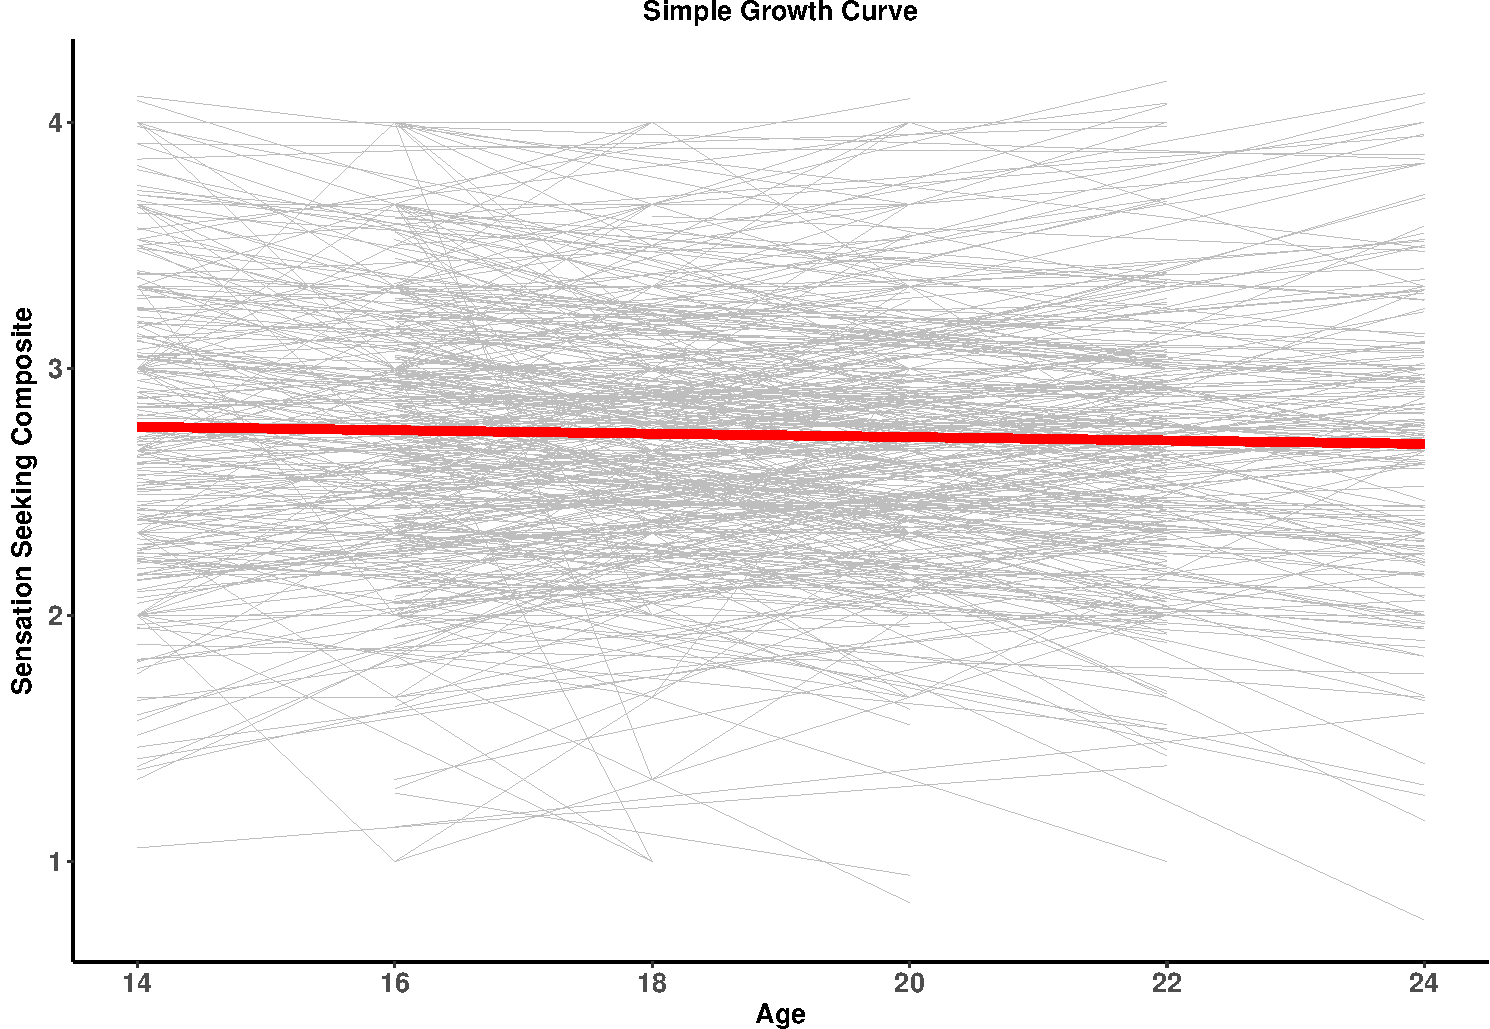
\includegraphics{Conditional_Models_files/figure-beamer/unnamed-chunk-3-1.pdf}

\end{frame}

\begin{frame}[fragile]{In R}

\small

\begin{Shaded}
\begin{Highlighting}[]
\NormalTok{mod0 <-}\StringTok{ }\KeywordTok{lmer}\NormalTok{(SensSeek ~}\StringTok{ }\NormalTok{age0 +}\StringTok{ }\NormalTok{(}\DecValTok{1}\NormalTok{|PROC_CID), }\DataTypeTok{data =} \NormalTok{sample_dat)}
\end{Highlighting}
\end{Shaded}

\centering
\tiny

\begin{verbatim}
## Linear mixed model fit by REML ['lmerMod']
## Formula: SensSeek ~ age0 + (1 | PROC_CID)
##    Data: sample_dat
## 
## REML criterion at convergence: 3404.2
## 
## Scaled residuals: 
##     Min      1Q  Median      3Q     Max 
## -3.6782 -0.5396  0.0276  0.4739  3.2174 
## 
## Random effects:
##  Groups   Name        Variance Std.Dev.
##  PROC_CID (Intercept) 0.1349   0.3673  
##  Residual             0.2003   0.4475  
## Number of obs: 2084, groups:  PROC_CID, 924
## 
## Fixed effects:
##              Estimate Std. Error t value
## (Intercept)  2.765851   0.020067  137.83
## age0        -0.005879   0.003407   -1.73
## 
## Correlation of Fixed Effects:
##      (Intr)
## age0 -0.611
\end{verbatim}

\normalsize
\raggedleft

\end{frame}

\begin{frame}{Conditional Models: Adding Predictors}

Let's see if we can better predict participants' change in sensation
seeking over time by adding covariates.

\begin{longtable}[]{@{}lll@{}}
\toprule
Predictor & Continuous & Categorical\tabularnewline
\midrule
\endhead
Time Invariant & Weight for Age & Group\tabularnewline
Time Varying & CESD Scores & Depression\tabularnewline
\bottomrule
\end{longtable}

\end{frame}

\section{Time Invariant Predictors}\label{time-invariant-predictors}

\begin{frame}{Time Invariant Predictors: Continuous}

The basic equation, specifying a random intercept and slope:\\

\begin{itemize}
  \item \textbf{Level 1:} $Y_{ij} = \beta_{0j} + \beta_{1j}*time_{1j} + \varepsilon{ij}$
  \item \textbf{Level 2:} 
    \begin{itemize} 
      \item $\beta_{0j} = \gamma_{00} + \gamma_{01}*X_{2j} + U_{0j}$
      \item $\beta_{1j} = \gamma_{10} + \gamma_{11}*X_{2j} + U_{1j}$
    \end{itemize}
\end{itemize}

But we need to break this down to see that adding additional predictors
results in interaction terms:

\(Y_{ij} = \gamma_{00} + \gamma_{01}*X_{2j} + U_{0j} + (\gamma_{10} + \gamma_{11}*X_{2j} + U_{1j})*X_{1j} + \varepsilon{ij}\)
\(Y_{ij} = \gamma_{00} + \gamma_{01}*X_{2j} + \gamma_{10}*X_{1j} + \textcolor{red}{\gamma_{11}*X_{2j}*X_{1j}} + U_{0j} + U_{1j}*X_{1j} + \varepsilon{ij}\)

We can also fit this with intercepts depending on weight, but without
the change (slope) dependent on weight:\\
\(Y_{ij} = \gamma_{00} + \gamma_{01}*X_{2j} + U_{0j} + (\gamma_{10} + U_{1j})*X_{1j} + \varepsilon{ij}\)
\(Y_{ij} = \gamma_{00} + \gamma_{01}*X_{2j} + \gamma_{10}*X_{1j} + U_{0j} + U_{1j}*X_{1j} + \varepsilon{ij}\)

\end{frame}

\begin{frame}[fragile]{Time Invariant Predictors: Continuous Example -
Weight for Age Percentile}

\begin{Shaded}
\begin{Highlighting}[]
\KeywordTok{describe}\NormalTok{(sample_dat$DemPweight)}
\end{Highlighting}
\end{Shaded}

\footnotesize

\begin{verbatim}
##    vars    n mean   sd median trimmed  mad   min  max range  skew kurtosis
## X1    1 2084 0.66 0.31   0.69    0.67 0.36 -0.06 1.62  1.68 -0.29    -0.56
##      se
## X1 0.01
\end{verbatim}

\normalsize

\end{frame}

\begin{frame}{Time Invariant Predictors: Continuous Example - Weight for
Age Percentile}

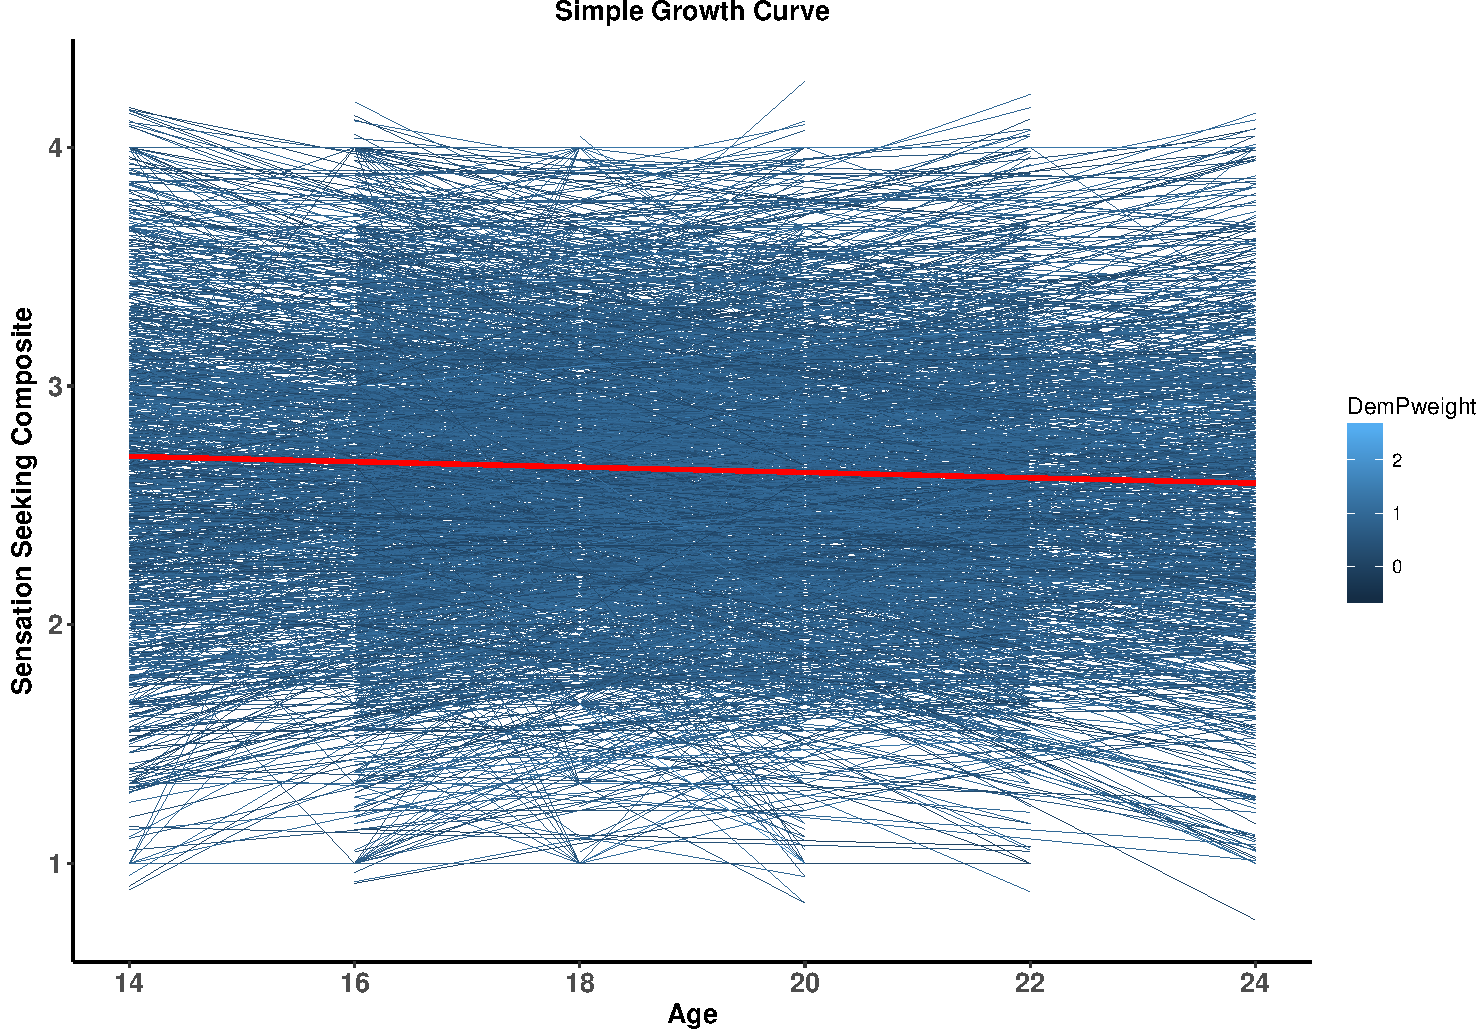
\includegraphics{Conditional_Models_files/figure-beamer/unnamed-chunk-8-1.pdf}

\end{frame}

\begin{frame}[fragile]{Time Invariant Predictors: Continuous Example -
Weight for Age Percentile}

\tiny

\begin{Shaded}
\begin{Highlighting}[]
\CommentTok{# time invariant covariate with random intecept (with weight as covariate) }
\CommentTok{# and slope (without weight as a covariate)}
\NormalTok{mod1a <-}\StringTok{ }\KeywordTok{lmer}\NormalTok{(SensSeek ~}\StringTok{ }\NormalTok{age0 +}\StringTok{ }\NormalTok{DemPweight +}\StringTok{ }\NormalTok{(age0|PROC_CID), }
              \DataTypeTok{data =} \NormalTok{sample_dat)}

\KeywordTok{summary}\NormalTok{(mod1a)}

\CommentTok{# time invariant predictor with random slope and intercept}
\NormalTok{mod1b <-}\StringTok{ }\KeywordTok{lmer}\NormalTok{(SensSeek ~}\StringTok{ }\NormalTok{age0 +}\StringTok{ }\NormalTok{DemPweight +}\StringTok{ }\NormalTok{age0*DemPweight +}\StringTok{ }
\StringTok{                }\NormalTok{(age0|PROC_CID), }\DataTypeTok{data =} \NormalTok{sample_dat)}

\KeywordTok{summary}\NormalTok{(mod1b)}
\end{Highlighting}
\end{Shaded}

\normalsize

\end{frame}

\begin{frame}{Time Invariant Predictors: Categorical Example - 2 level
group}

Lets's start with 2 groups: Jail v. None

\begin{itemize}
  \item \textbf{Level 1:} $Y_{ij} = \beta_{0j} + \beta_{1j}*time_{1j} + \varepsilon{ij}$
  \item \textbf{Level 2:} 
    \begin{itemize} 
      \item $\beta_{0j} = \gamma_{00} + \gamma_{01}*X_{2j} + U_{0j}$
      \item $\beta_{1j} = \gamma_{10} + \gamma_{11}*X_{2j} + U_{1j}$
    \end{itemize}
\end{itemize}

\end{frame}

\begin{frame}{Time Invariant Predictors: Example - 2 level group}

\begin{itemize}
  \item \textbf{Level 1:} $Y_{ij} = \beta_{0j} + \beta_{1j}*age0_{ij} + \varepsilon{ij}$
  \item \textbf{Level 2:} 
    \begin{itemize} 
      \item $\beta_{0j} = \gamma_{00} + \gamma_{01}*groupsNone + U_{0j}$
      \item $\beta_{1j} = \gamma_{10} + \gamma_{11}*groupsNone + U_{1j}$
    \end{itemize}
\end{itemize}

\begin{longtable}[]{@{}ll@{}}
\toprule
Variable & D1\tabularnewline
\midrule
\endhead
Jail & 0\tabularnewline
None & 1\tabularnewline
\bottomrule
\end{longtable}

\end{frame}

\begin{frame}

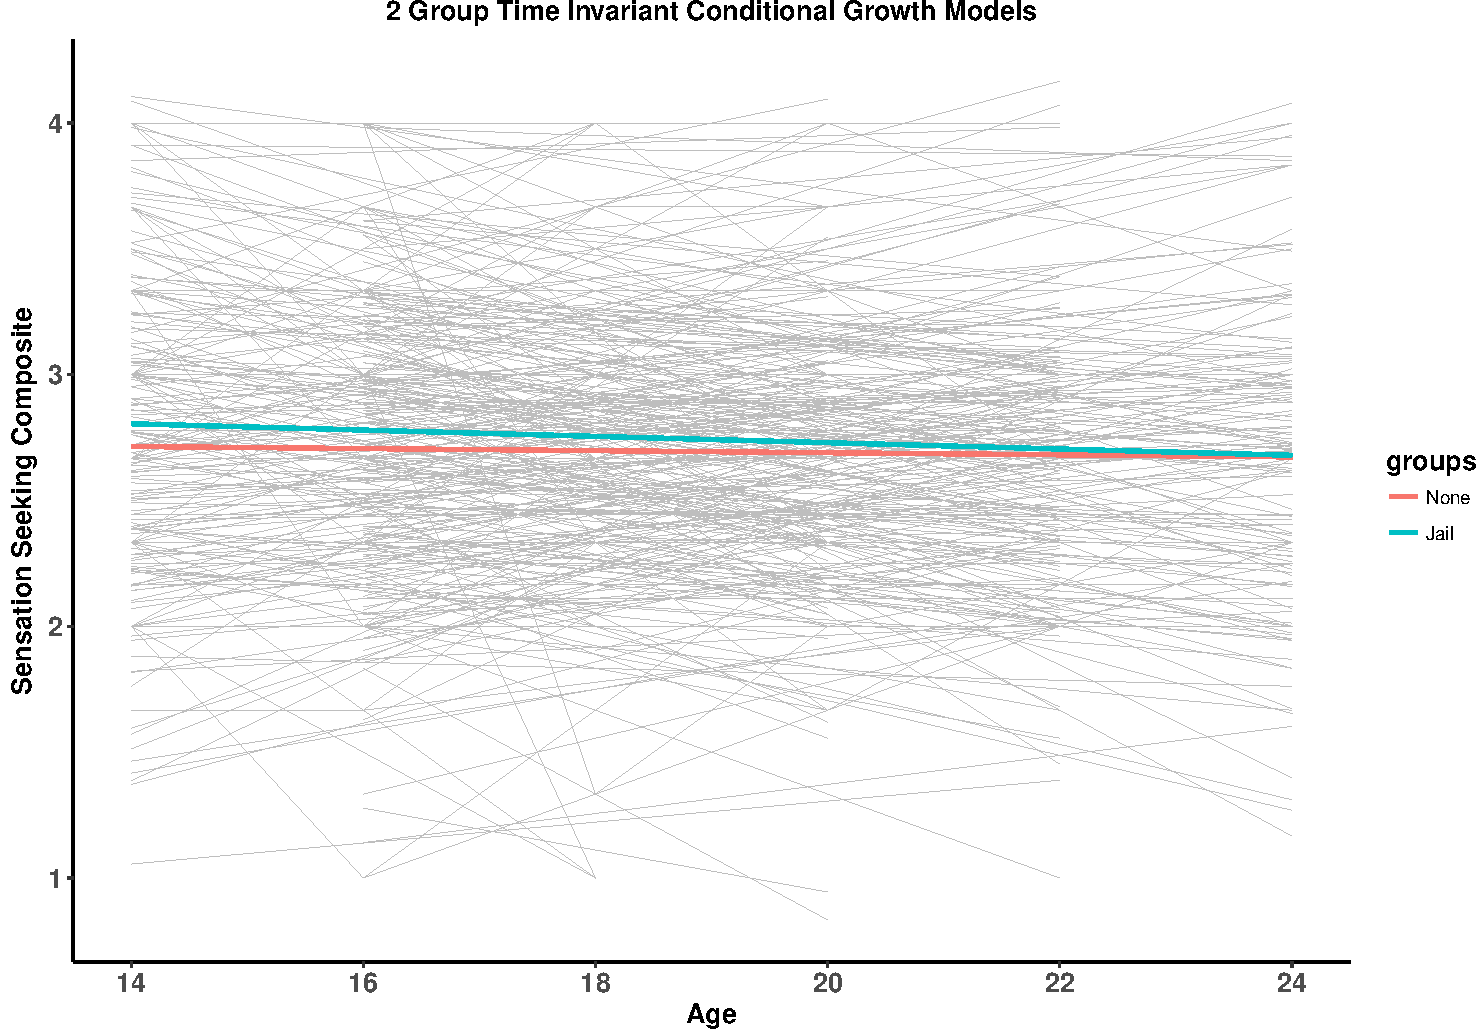
\includegraphics{Conditional_Models_files/figure-beamer/unnamed-chunk-10-1.pdf}

\end{frame}

\begin{frame}[fragile]{Time Invariant Predictors: Example - 2 level
group}

\tiny

\begin{Shaded}
\begin{Highlighting}[]
\NormalTok{mod2g <-}\StringTok{ }\KeywordTok{lmer}\NormalTok{(SensSeek ~}\StringTok{ }\NormalTok{age0 +}\StringTok{ }\NormalTok{groups +}\StringTok{ }\NormalTok{age0*groups +}\StringTok{ }\NormalTok{(age0|PROC_CID), }
              \DataTypeTok{data =} \NormalTok{sample_dat %>%}\StringTok{ }\KeywordTok{filter}\NormalTok{(groups !=}\StringTok{ "CommServ"}\NormalTok{))}
\KeywordTok{summary}\NormalTok{(mod2g)}
\end{Highlighting}
\end{Shaded}

\tiny

\begin{verbatim}
## Linear mixed model fit by REML ['lmerMod']
## Formula: SensSeek ~ age0 + groups + age0 * groups + (age0 | PROC_CID)
##    Data: sample_dat %>% filter(groups != "CommServ")
## 
## REML criterion at convergence: 2607.6
## 
## Scaled residuals: 
##     Min      1Q  Median      3Q     Max 
## -3.2324 -0.4860  0.0463  0.4643  3.0578 
## 
## Random effects:
##  Groups   Name        Variance  Std.Dev. Corr 
##  PROC_CID (Intercept) 0.1613721 0.40171       
##           age0        0.0008963 0.02994  -0.31
##  Residual             0.1897644 0.43562       
## Number of obs: 1573, groups:  PROC_CID, 689
## 
## Fixed effects:
##                  Estimate Std. Error t value
## (Intercept)      2.717417   0.036423   74.61
## age0            -0.003998   0.006382   -0.63
## groupsJail       0.093497   0.048257    1.94
## age0:groupsJail -0.007432   0.008272   -0.90
## 
## Correlation of Fixed Effects:
##             (Intr) age0   grpsJl
## age0        -0.624              
## groupsJail  -0.755  0.471       
## age0:grpsJl  0.481 -0.772 -0.623
\end{verbatim}

\normalsize

\end{frame}

\begin{frame}[fragile]{Side Note: \texttt{lme4} helper functions}

\begin{Shaded}
\begin{Highlighting}[]
\KeywordTok{vcov}\NormalTok{(mod2g)}
\KeywordTok{VarCorr}\NormalTok{(mod2g)}
\KeywordTok{fixef}\NormalTok{(mod2g)}
\KeywordTok{ranef}\NormalTok{(mod2g)}
\KeywordTok{coef}\NormalTok{(mod2g)}
\KeywordTok{confint.merMod}\NormalTok{(mod2g, }\DataTypeTok{method =} \StringTok{"boot"}\NormalTok{)}
\NormalTok{reghelper::}\KeywordTok{ICC}\NormalTok{(mod2g)}
\NormalTok{MuMIn::}\KeywordTok{r.squaredGLMM}\NormalTok{(mod2g)}
\end{Highlighting}
\end{Shaded}

\end{frame}

\begin{frame}[fragile]

\small

\begin{Shaded}
\begin{Highlighting}[]
\KeywordTok{vcov}\NormalTok{(mod2g)}
\end{Highlighting}
\end{Shaded}

\begin{verbatim}
## 4 x 4 Matrix of class "dpoMatrix"
##                   (Intercept)          age0    groupsJail age0:groupsJail
## (Intercept)      0.0013266680 -1.449788e-04 -0.0013266680    1.449788e-04
## age0            -0.0001449788  4.072833e-05  0.0001449788   -4.072833e-05
## groupsJail      -0.0013266680  1.449788e-04  0.0023287011   -2.486054e-04
## age0:groupsJail  0.0001449788 -4.072833e-05 -0.0002486054    6.842322e-05
\end{verbatim}

\end{frame}

\begin{frame}[fragile]

\small

\begin{Shaded}
\begin{Highlighting}[]
\KeywordTok{VarCorr}\NormalTok{(mod2g)}
\end{Highlighting}
\end{Shaded}

\begin{verbatim}
##  Groups   Name        Std.Dev. Corr  
##  PROC_CID (Intercept) 0.401711       
##           age0        0.029938 -0.313
##  Residual             0.435620
\end{verbatim}

\end{frame}

\begin{frame}[fragile]

\small

\begin{Shaded}
\begin{Highlighting}[]
\KeywordTok{fixef}\NormalTok{(mod2g)}
\end{Highlighting}
\end{Shaded}

\begin{verbatim}
##     (Intercept)            age0      groupsJail age0:groupsJail 
##     2.717416961    -0.003997618     0.093496648    -0.007431764
\end{verbatim}

\end{frame}

\begin{frame}[fragile]

\small

\begin{Shaded}
\begin{Highlighting}[]
\KeywordTok{ranef}\NormalTok{(mod2g)}
\end{Highlighting}
\end{Shaded}

\begin{verbatim}
## $PROC_CID
##          (Intercept)          age0
## 9102     0.282588931 -3.611031e-03
## 9501     0.158291229  1.331088e-03
## 9502     0.154297404 -3.923893e-04
## 9503     0.141135024  2.529397e-04
## 10001    0.181445259 -8.900323e-04
## 12802    0.299965270 -2.762459e-03
## 13801    0.295128758 -6.380208e-03
## 14302    0.457651355 -3.128200e-03
## 17502    0.059294263  7.862636e-03
## 18301   -0.005625690  6.023488e-03
## 18801    0.051321841  4.697355e-04
## 22901   -0.170342105  2.176698e-03
## 23603   -0.023323357  5.432364e-04
## 29201    0.236336994 -5.180336e-05
## 37902    0.399042993 -7.794982e-03
## 38803    0.129866933 -3.024798e-03
## 42801    0.131611919 -1.681788e-03
## 43902   -0.170342105  2.176698e-03
## 47201   -0.205957485  2.631805e-03
## 47402    0.024527633 -1.784607e-03
## 49201    0.085910217 -3.799037e-03
## 50701    0.006921081  1.140965e-02
## 50702    0.061796677 -3.925860e-03
## 54601    0.078141277 -2.900301e-02
## 56301   -0.036390273  3.182226e-03
## 57603   -0.019365093  2.474547e-04
## 58502    0.102444274 -1.214135e-04
## 58803   -0.094454894  7.314253e-03
## 58901    0.073515798 -1.084984e-02
## 59004   -0.151087599  3.119537e-03
## 62102   -0.783987879  1.435328e-03
## 63203   -0.258333216  7.701070e-03
## 65601   -0.332526865  1.363306e-03
## 71301    0.383931790  4.861444e-04
## 71302    0.521935007  5.857198e-03
## 73303    0.391191647 -4.688189e-03
## 74301   -0.205957485  2.631805e-03
## 74302    0.095996539 -1.226681e-03
## 75201    0.210826536  6.425101e-03
## 75503    0.073876655  1.028040e-03
## 75702    0.131611919 -1.681788e-03
## 76102    0.239927758 -5.625604e-03
## 76803   -0.157493850  1.071256e-02
## 77001   -0.025538134 -1.182362e-02
## 82802    0.017733952  1.221525e-03
## 82901    0.254884826 -2.896596e-03
## 82902    0.086898597 -2.024000e-03
## 83601    0.258646995 -1.376925e-03
## 83602    0.254884826 -2.896596e-03
## 83603    0.126321826 -2.175315e-03
## 85603    0.164144127  2.039530e-03
## 90602    0.095996539 -1.226681e-03
## 91801   -0.157678825 -6.492841e-03
## 93503    0.067279101  3.087615e-03
## 94902   -0.211332882 -7.282256e-03
## 96702    0.129866933 -3.024798e-03
## 101504   0.095996539 -1.226681e-03
## 102505   0.022070641  6.991307e-03
## 104001  -0.302594836  1.510746e-03
## 105703  -0.537629765  1.028239e-03
## 110401   0.234909700 -5.572155e-03
## 115801   0.162493828  1.124937e-02
## 117702   0.095996539 -1.226681e-03
## 117902   0.141135024  2.529397e-04
## 121601   0.072632926  3.350792e-03
## 122402  -0.166680521 -2.325491e-04
## 124402  -0.437596780  6.420519e-03
## 124403  -0.471212888  4.538533e-03
## 124601   0.610881699  1.239881e-02
## 126101  -0.010152672 -5.491056e-03
## 129501  -0.719397240  1.331429e-02
## 130602   0.027164610 -2.891933e-03
## 132601   0.282588931 -3.611031e-03
## 137603  -0.575171746 -8.807449e-03
## 140201  -0.205957485  2.631805e-03
## 140901  -0.309338679  4.237268e-02
## 141201   0.379894995 -6.191271e-03
## 141401  -0.123004905 -5.171472e-03
## 141502  -0.295881296  1.227209e-02
## 141506   0.162197026  3.196930e-03
## 141601   0.126321826 -2.175315e-03
## 141902   0.744320675 -5.568256e-03
## 143502  -0.338253957  3.550824e-03
## 143602  -0.040641146 -5.026486e-03
## 143901   0.017733952  1.221525e-03
## 149801   0.148949173 -7.197339e-03
## 151903   0.096548003 -9.166118e-03
## 152503   0.176808828 -3.934445e-03
## 153301  -0.201555245  1.323707e-02
## 153801   0.002718482  1.491363e-03
## 154102   0.158291229  1.331088e-03
## 155101  -0.200818956  2.061711e-02
## 156604   0.569423477 -4.539559e-03
## 157102   0.052118297 -2.664992e-03
## 158402   0.741727842  1.577046e-03
## 159605  -0.025145656  8.672515e-03
## 159606   0.040242176 -5.783045e-03
## 160502   0.131611919 -1.681788e-03
## 165601   0.029121461  5.939693e-03
## 170404  -0.027245435  4.741542e-04
## 170405   0.086898597 -2.024000e-03
## 172303   0.275699138 -3.267492e-04
## 172902   0.095996539 -1.226681e-03
## 172903   0.095996539 -1.226681e-03
## 173301   0.089715265 -4.508307e-03
## 173302  -0.066291692  1.544034e-03
## 173503   0.283057222 -6.592832e-03
## 175201  -0.295467749 -6.995329e-03
## 182901  -0.458135321  1.647421e-03
## 188001  -0.150648231 -2.433387e-03
## 189602   0.131611919 -1.681788e-03
## 196202   0.092012175 -2.979851e-03
## 198601   0.141135024  2.529397e-04
## 200208   0.092012175 -2.979851e-03
## 201302  -0.415416081  5.168146e-05
## 204601   0.095996539 -1.226681e-03
## 205701   0.294068782  2.162961e-02
## 206301   0.217338200 -3.073484e-03
## 209402   0.116745250 -9.047318e-03
## 210202   0.125121059  1.641771e-03
## 210504   0.095996539 -1.226681e-03
## 211903   0.099104138 -5.059686e-03
## 213002  -0.359110634 -2.587132e-02
## 213402   0.007395556 -6.058809e-03
## 224001   0.193478771 -4.357028e-03
## 224901   0.382083408 -3.066210e-03
## 225003  -0.106616062  9.558863e-03
## 225301  -0.590826727 -4.950214e-03
## 225302  -0.396236503  5.790491e-03
## 226701  -0.389489802  5.441921e-03
## 226704  -0.501785084 -9.189436e-03
## 231102   0.264859327 -3.174392e-03
## 231902   0.162197026  3.196930e-03
## 231903  -0.080660508 -6.593366e-03
## 231904   0.358167714 -9.778510e-03
## 233301   0.131856410 -1.232128e-03
## 234701  -0.376962791  1.265639e-02
## 239604   0.014087043 -8.211848e-07
## 239901   0.407773467 -1.040304e-02
## 240002   0.282588931 -3.611031e-03
## 243701   0.126321826 -2.175315e-03
## 245903   0.408185205  9.006733e-03
## 246202  -0.001408447 -1.369982e-02
## 247801  -0.043608500  1.252834e-02
## 248501   0.414165374 -1.702551e-02
## 249203   0.584542955 -7.469517e-03
## 249601   0.334398839  7.691337e-04
## 252502  -0.127383150  6.329571e-03
## 253802   0.181028902 -6.192015e-05
## 254402   0.085910217 -3.799037e-03
## 254902   0.498434441 -4.997219e-03
## 255902   0.322477370 -2.970244e-02
## 259903  -0.110864825 -2.375115e-02
## 260601   0.126321826 -2.175315e-03
## 262601  -0.205957485  2.631805e-03
## 262602  -0.066291692  1.544034e-03
## 265202  -0.054980473  7.025619e-04
## 265403  -0.658888522  8.419534e-03
## 265504   0.095996539 -1.226681e-03
## 266201  -0.237701047  1.577368e-02
## 266304   0.061731183  5.339498e-03
## 266401  -1.006320743  3.753192e-03
## 267902  -0.080972044  1.939503e-03
## 268303   0.158291229  1.331088e-03
## 269101  -0.036645584  3.154889e-03
## 269202   0.113890470  1.227100e-02
## 270601   0.241703381 -8.578287e-03
## 272201   0.391373432 -1.693083e-04
## 272901   0.749434610 -4.418729e-04
## 275802   0.256212883  1.332746e-04
## 279501  -0.091373773 -1.870776e-03
## 285502  -0.862530628  9.154618e-03
## 286401   0.129866933 -3.024798e-03
## 287803  -0.241653064  3.541904e-03
## 287804  -0.209548512 -6.895443e-04
## 287805  -0.060269368 -4.616167e-03
## 287902   0.126321826 -2.175315e-03
## 288602   0.076187810 -2.405090e-03
## 291102   0.343497575 -8.968996e-03
## 293801   0.129866933 -3.024798e-03
## 294801  -0.094326257 -2.567075e-03
## 295902   0.131611919 -1.681788e-03
## 302001  -0.016001889 -5.444977e-03
## 304301  -0.224504155  4.012882e-04
## 304604  -0.327417820  2.049786e-03
## 304901  -0.108446901 -7.161039e-03
## 305103   0.086898597 -2.024000e-03
## 306601   0.245434080  2.137691e-03
## 307501   0.033218827 -2.771276e-03
## 310103  -0.057392997 -7.005532e-03
## 311301   0.296759346 -1.701896e-02
## 317901   0.378832325  3.878484e-04
## 318201   0.086898597 -2.024000e-03
## 320103  -0.036382930  3.573418e-03
## 324302   0.031160171  5.289442e-03
## 325001   0.059294263  7.862636e-03
## 325002   0.202008820 -7.296163e-03
## 325003   0.095996539 -1.226681e-03
## 325004   0.240088886 -5.592034e-03
## 325201   0.746026230  8.522044e-03
## 325301   0.389602461 -2.715154e-03
## 325901   0.134195255 -1.181757e-02
## 325902  -0.127371019 -6.703673e-03
## 326002  -0.672279236  7.972764e-03
## 330602  -0.019690667  2.275097e-04
## 331201  -0.098110168 -4.576554e-03
## 331505  -0.649966880 -1.602738e-02
## 332201   0.282588931 -3.611031e-03
## 334101   0.433565943 -5.540274e-03
## 335502   0.273487078  2.687283e-03
## 335503   0.029443169  1.409325e-03
## 336001  -0.219481982  5.112068e-03
## 337002  -0.023323357  5.432364e-04
## 337104  -0.399736324  8.203405e-03
## 338702  -0.049007184  5.711611e-03
## 342303  -0.170342105  2.176698e-03
## 344702   0.040213305 -1.693677e-03
## 344703   0.057610281 -4.012274e-03
## 345602   0.336703894 -5.962864e-03
## 345801  -0.122247035 -6.138344e-04
## 346502  -0.402537609 -5.434574e-03
## 348604  -0.205957485  2.631805e-03
## 349101  -0.450095920 -5.798363e-03
## 351101  -0.478220030  2.012281e-02
## 351102   0.260943232  5.550212e-03
## 354503   0.182708635 -1.254026e-03
## 354902   0.084646790 -2.074963e-03
## 355502   0.182708635 -1.254026e-03
## 356402  -0.054980473  7.025619e-04
## 356501  -0.074241007  1.077038e-02
## 358401  -0.253301418 -2.685357e-04
## 359402   0.081892799  2.133732e-03
## 360102   0.384667715 -5.320773e-03
## 361401   0.296907540 -2.733858e-03
## 363502  -0.287291689  1.014991e-02
## 363703  -0.238194595 -1.847721e-02
## 365404  -0.054980473  7.025619e-04
## 365405   0.397950563 -5.085167e-03
## 365406   0.095996539 -1.226681e-03
## 366201   0.014087043 -8.211848e-07
## 368701  -0.170342105  2.176698e-03
## 369803   0.129866933 -3.024798e-03
## 370302  -0.166680521 -2.325491e-04
## 371402   0.329312276 -1.452370e-05
## 371403  -0.132264925  3.474996e-02
## 372802  -0.175480257 -5.904342e-03
## 372803  -0.254718055  8.051080e-03
## 372902  -0.533797727  2.267529e-03
## 373401  -0.321319117  4.105941e-03
## 377102   0.131611919 -1.681788e-03
## 379801  -0.359805935  7.034903e-03
## 381401  -0.170342105  2.176698e-03
## 382302  -0.307868606 -5.383323e-03
## 383602   0.240088886 -5.592034e-03
## 383703   0.400873165 -1.326793e-02
## 385901   0.067279101  3.087615e-03
## 387901   0.232859988 -1.136632e-02
## 390801   0.086898597 -2.024000e-03
## 390802   0.457651355 -3.128200e-03
## 393104  -0.117038508  1.178908e-02
## 398201   0.281584795 -1.028464e-02
## 399801  -0.356934497  4.561048e-03
## 401202  -0.290584044 -8.662447e-03
## 402402   0.327329364 -2.496263e-04
## 402803   0.539535642  2.818446e-03
## 404503   0.506556441 -1.341078e-02
## 405702   0.095996539 -1.226681e-03
## 411002  -0.156332257 -6.308186e-03
## 417001  -0.259823653  7.902867e-04
## 419402  -0.190499059 -1.735555e-02
## 419403   0.131856410 -1.232128e-03
## 420001   0.035793521 -2.924148e-03
## 421802   0.095996539 -1.226681e-03
## 425602  -0.652887080  6.150245e-03
## 427201   0.282588931 -3.611031e-03
## 427402  -0.107058839 -7.439650e-03
## 427703   0.341835578  2.211051e-02
## 429002  -0.150648231 -2.433387e-03
## 433902  -0.019365093  2.474547e-04
## 434501   0.543831561  1.844243e-02
## 436702   0.533200728 -4.292610e-04
## 439602   0.095722601 -1.047018e-02
## 444502   0.279617901 -8.964062e-03
## 444703   0.073876655  1.028040e-03
## 446501   0.392903782 -2.381160e-03
## 446502   0.240088886 -5.592034e-03
## 447301   0.558408331  1.726013e-02
## 448304  -0.536367689 -2.244931e-02
## 448702   0.488727331  1.494105e-02
## 449002  -0.010581807 -9.519387e-03
## 449902  -0.286282637  5.152519e-03
## 449903  -0.084060242  1.612234e-03
## 452801   0.393279175 -9.160069e-03
## 453701   0.027385223  3.402475e-03
## 453702  -0.484290454  7.429645e-03
## 458902  -0.091373773 -1.870776e-03
## 465002  -0.066291692  1.544034e-03
## 468902  -0.170342105  2.176698e-03
## 471101  -0.472296129  6.035184e-03
## 474103   0.700311762 -3.674664e-03
## 474503   0.318186036  3.663231e-03
## 474601   0.251295348 -1.063045e-02
## 475301   0.027385223  3.402475e-03
## 475302  -0.166680521 -2.325491e-04
## 478403   0.039350951 -1.820944e-02
## 478701   0.242980331  1.210182e-02
## 478702   0.265099789 -1.468775e-03
## 484201   0.168102369  2.223586e-03
## 487002   0.086898597 -2.024000e-03
## 487101   0.294778704 -3.211456e-03
## 491903   0.485389813  7.490079e-04
## 492502  -0.253556739  9.020536e-03
## 495003   0.039284357  1.898974e-03
## 495004  -0.241189083 -1.475486e-02
## 495401   0.445291768 -9.359704e-03
## 495402  -0.066291692  1.544034e-03
## 495403  -0.066291692  1.544034e-03
## 495801  -0.719397240  1.331429e-02
## 497303  -0.121524468 -4.269927e-03
## 497602  -0.070472881 -4.400030e-03
## 498102  -0.189964753 -1.745354e-02
## 498103   0.129866933 -3.024798e-03
## 502602  -0.054980473  7.025619e-04
## 504901   0.072632926  3.350792e-03
## 506301  -0.295619022 -5.497902e-03
## 506402   0.103884108 -1.408874e-03
## 509101  -0.023323357  5.432364e-04
## 509602   0.095996539 -1.226681e-03
## 509603  -0.372672271  8.680102e-03
## 510001   0.406701257 -2.931289e-02
## 510301   0.367771025 -6.279059e-04
## 512504   0.470161772  2.969041e-03
## 513401   0.764930854  5.828978e-03
## 513403   0.086898597 -2.024000e-03
## 513404  -0.205957485  2.631805e-03
## 513405  -0.205957485  2.631805e-03
## 513502  -0.057246207 -1.401062e-02
## 515201   0.357006120  7.242232e-03
## 516403   0.295128758 -6.380208e-03
## 521601   0.118499046 -8.941106e-04
## 524701  -0.077610631 -1.961224e-02
## 531001   0.138275150 -8.727404e-04
## 533001  -0.028698830  8.579603e-03
## 534902   0.181028902 -6.192015e-05
## 539701   0.177818188  1.148858e-03
## 540802   0.312221521 -1.234542e-02
## 542101  -0.497220965  9.993096e-03
## 544201  -0.077266561 -1.393898e-03
## 548002   0.068815232  5.024844e-03
## 548803   0.567792983 -1.437347e-02
## 553701   0.311465198  2.755167e-03
## 554702   0.481622753  1.531421e-02
## 555001  -0.215485356 -6.222561e-04
## 556101  -0.364013006 -3.577905e-03
## 557601   0.027385223  3.402475e-03
## 561501  -0.202503282  2.352664e-05
## 563102  -0.086364579  6.552010e-03
## 564601   0.246533716  8.579136e-03
## 565602   0.084646790 -2.074963e-03
## 567002  -0.356934497  4.561048e-03
## 576702  -0.066291692  1.544034e-03
## 576901   0.178547873  7.720089e-03
## 577301  -0.191131081 -1.898210e-03
## 579802  -0.320946172 -2.492211e-03
## 580301  -0.378299146 -1.006186e-02
## 581101  -0.303673435  9.895425e-03
## 581902   0.087505473 -1.114904e-03
## 582102   0.391174886 -7.007811e-03
## 584102  -0.333539904 -6.890430e-03
## 584401   0.095996539 -1.226681e-03
## 585204   0.131611919 -1.681788e-03
## 585501  -0.144248532  8.446979e-03
## 586103   0.684311707  1.313807e-02
## 586202   0.106907835  5.859555e-03
## 587303   0.567386255 -1.235968e-02
## 589702  -0.108453505 -9.288276e-03
## 593206   0.017733952  1.221525e-03
## 594103  -0.448742977  6.232362e-03
## 595102   0.138275150 -8.727404e-04
## 597305   0.095996539 -1.226681e-03
## 598001  -0.116534745 -1.671428e-02
## 600702  -0.143753274 -1.387989e-02
## 600703  -0.230641659  1.526674e-02
## 602303   0.013903716  1.782110e-02
## 603002  -0.253301418 -2.685357e-04
## 604704  -0.349619628  7.328516e-03
## 608405   0.608350634 -1.380149e-02
## 610704  -0.199771080 -5.666178e-03
## 615401  -0.313520882 -2.516643e-03
## 620902  -0.173145224  6.651133e-03
## 621701  -0.184003506  2.511726e-02
## 623202  -0.445165408  4.875728e-04
## 623403  -0.343649045  1.500523e-03
## 627002   0.498434441 -4.997219e-03
## 627403  -0.437972841  3.129359e-03
## 627404  -0.525862560  1.224814e-02
## 627701   0.088712655 -1.252777e-02
## 628201  -0.378299146 -1.006186e-02
## 628205  -0.188440870  1.060796e-02
## 629305   0.149045285 -3.975743e-03
## 629403   0.081892799  2.133732e-03
## 629703  -0.285249981  1.448676e-02
## 629902  -0.224504155  4.012882e-04
## 631002   0.093709924 -3.700065e-02
## 631203  -0.036382930  3.573418e-03
## 632201  -0.624501595  8.731522e-05
## 633402  -0.341765511  4.745544e-03
## 633603  -0.660735453  1.192993e-02
## 634501  -0.381094478 -6.166064e-03
## 636302  -0.233777076 -5.627336e-03
## 636402   0.091668875  1.238787e-02
## 638001  -0.050755272  5.737782e-03
## 647202  -0.338253957  3.550824e-03
## 648201  -0.260851737  1.502780e-02
## 651501   0.095996539 -1.226681e-03
## 651604  -0.055792564  6.528123e-04
## 665201   0.131856410 -1.232128e-03
## 667602  -0.772184029  2.184108e-02
## 667603  -0.337328531  9.571297e-03
## 670902  -0.167375630 -1.138029e-03
## 674402  -0.283938246 -6.245952e-03
## 674502   0.323982188  2.151910e-03
## 675601  -0.257869371  7.992941e-03
## 677301   0.343036007 -6.016892e-03
## 677302   0.138992467  1.460947e-02
## 682903  -0.170342105  2.176698e-03
## 684703  -0.199160738 -4.231207e-03
## 685806  -0.245835230 -5.743808e-03
## 686203  -0.437972841  3.129359e-03
## 688002  -0.066291692  1.544034e-03
## 695302  -0.039449012 -1.274014e-02
## 696602  -0.054980473  7.025619e-04
## 696603  -0.023323357  5.432364e-04
## 698901  -0.322389655  1.105678e-02
## 698902   0.464633019 -2.714304e-02
## 699502   0.111220499 -4.349865e-03
## 699503  -0.565104036  2.888185e-02
## 706402  -0.023323357  5.432364e-04
## 706603  -0.495702474 -4.594660e-03
## 708402   0.208904939 -1.428635e-03
## 708901   0.015836434  7.425121e-03
## 710502   0.204248906 -7.460031e-03
## 711501  -0.216396656  8.210985e-03
## 713902   0.514882464  9.158826e-03
## 714402   0.315881713 -7.173042e-04
## 715203  -0.166680521 -2.325491e-04
## 715601   0.088767018  2.457669e-03
## 715602  -1.108491127  8.083249e-03
## 717003  -0.373574346  1.228579e-03
## 718403   0.067279101  3.087615e-03
## 718404  -0.170342105  2.176698e-03
## 718903   0.138275150 -8.727404e-04
## 719401  -0.017314397  8.676060e-05
## 722803  -0.023323357  5.432364e-04
## 723502  -0.224504155  4.012882e-04
## 723602  -0.349619628  7.328516e-03
## 724603   0.546469464 -1.272810e-02
## 724903  -0.019365093  2.474547e-04
## 725601  -0.556181289 -1.970179e-03
## 727601  -0.030437492 -1.015735e-02
## 727804  -0.755735967  9.314510e-03
## 728201  -0.276306946 -2.835174e-03
## 731603  -0.019365093  2.474547e-04
## 731702   0.131856410 -1.232128e-03
## 732302  -0.482712816 -9.790925e-04
## 732503  -0.140401087  4.747345e-03
## 732505   0.131611919 -1.681788e-03
## 739101   0.196283632  3.261211e-03
## 742301  -0.219481982  5.112068e-03
## 743303  -0.848855998  2.054019e-02
## 743802  -0.115461365 -1.202409e-02
## 744102  -0.432608138 -4.653857e-03
## 744602  -0.219481982  5.112068e-03
## 744703  -0.205957485  2.631805e-03
## 744805  -0.504824377  9.187331e-03
## 744903  -0.176513646  4.111271e-03
## 745506  -0.329703935  7.679305e-03
## 745901   0.057315304 -4.927817e-04
## 746404   0.126378815  1.900572e-04
## 747902  -0.060269368 -4.616167e-03
## 748502   0.191258610  1.213281e-02
## 749701  -0.269083398 -1.361868e-02
## 750103  -0.235946474 -2.211357e-03
## 754802  -0.620715531 -3.712752e-03
## 757802   0.182708635 -1.254026e-03
## 758302  -0.589336383 -1.772575e-02
## 760101   0.346457174  1.207741e-02
## 760301   0.173999138 -2.141309e-04
## 762201   0.076178863 -2.622437e-03
## 765701   0.087867569  3.314291e-03
## 767301  -0.395770280 -8.122125e-03
## 768701  -0.339910996  3.950296e-03
## 771002  -0.057886106 -3.109417e-02
## 775002   0.043852691  1.808749e-03
## 779101  -0.034955326  3.310105e-03
## 779401  -0.090445753 -2.771444e-03
## 781002   0.086898597 -2.024000e-03
## 781403   0.329216619  3.106280e-02
## 781901  -0.176321422  8.178305e-03
## 782301   0.169063304  3.219972e-03
## 788602  -0.023568018  2.637773e-04
## 789101   0.038113084 -3.752456e-03
## 792801  -0.176529670 -9.380617e-03
## 793303  -0.015165611  1.797376e-05
## 793802  -0.838778380  1.805038e-02
## 795001   0.131856410 -1.232128e-03
## 795101  -0.372672271  8.680102e-03
## 795201   0.007189141 -2.889615e-03
## 796703  -0.334923592  1.415345e-02
## 796805   0.095996539 -1.226681e-03
## 797103   0.154297404 -3.923893e-04
## 798003   0.095996539 -1.226681e-03
## 799702  -0.023323357  5.432364e-04
## 802001  -0.451462734  5.350582e-04
## 804403   0.300403056 -5.914631e-03
## 809102  -0.289935221 -3.718354e-03
## 809105  -0.019365093  2.474547e-04
## 809302  -0.219481982  5.112068e-03
## 810302  -0.238654652  3.706351e-03
## 810903   0.053319742 -8.674157e-03
## 814101   0.191684613  1.204741e-02
## 814302   0.243659442  6.206137e-04
## 815202   0.078998624 -2.829554e-03
## 817406  -0.205957485  2.631805e-03
## 819502   0.352583106  1.062427e-02
## 821003  -0.566607110  1.292325e-02
## 821004   0.071147132  6.139801e-03
## 825902  -0.110754353 -2.748247e-03
## 826101  -0.921861661 -7.860999e-03
## 826502  -0.428589753 -3.287131e-04
## 826902  -0.836854088  1.594566e-02
## 827901   0.907030440  2.365059e-03
## 828905  -0.219481982  5.112068e-03
## 829602   0.366721585  1.455853e-02
## 829604   0.125799743  1.467280e-03
## 830501   0.168102369  2.223586e-03
## 830504   0.251399545 -3.098214e-02
## 830902  -0.248776697  3.463819e-03
## 831501  -0.306867922 -3.095220e-03
## 833001   0.042660099  1.080707e-02
## 835704  -0.122247035 -6.138344e-04
## 837402   0.095996539 -1.226681e-03
## 837502   0.295696107 -2.157037e-02
## 839101   0.844863501  7.358151e-03
## 842204   0.282588931 -3.611031e-03
## 847701   0.158291229  1.331088e-03
## 850201  -0.416484699  9.564198e-03
## 850502  -0.124081643 -2.531395e-03
## 851003   0.368634628 -6.046131e-03
## 851004  -0.296368678  1.343029e-04
## 853201  -0.295619022 -5.497902e-03
## 859806  -0.458430639 -8.004772e-04
## 861503   0.162776120  1.377173e-03
## 861901  -0.448782014 -9.909214e-03
## 863401   0.528426478  6.934976e-03
## 863901   0.304350976 -1.503153e-02
## 864102  -0.096462415  9.339591e-03
## 864902   0.035793521 -2.924148e-03
## 866206   0.327319034 -1.451654e-02
## 869604  -0.158865716 -7.671699e-03
## 870503   0.147455628  3.040195e-03
## 870601  -0.301852549  9.813742e-03
## 870602   0.066755129  4.799024e-03
## 870604   0.443230820 -1.512932e-03
## 870803  -0.176513646  4.111271e-03
## 879403   0.278035995 -4.149979e-04
## 891602   0.329910214 -2.956732e-03
## 892001  -0.051680175 -1.237358e-02
## 892002  -0.042988100  5.094803e-05
## 892502   0.191669782 -2.208036e-03
## 892601  -0.387665653 -3.355812e-03
## 894202   0.181973106 -2.107017e-03
## 894601  -0.050753899  5.737692e-03
## 894602   0.085888360  1.031511e-02
## 895301   0.582848860 -8.404933e-03
## 896203   0.129866933 -3.024798e-03
## 898501   0.093209577 -4.542002e-03
## 901904   0.240088886 -5.592034e-03
## 904501  -0.121524468 -4.269927e-03
## 904502  -0.344442753  9.762109e-04
## 904804  -0.055699839  1.985751e-02
## 904805  -0.143684039  9.693673e-03
## 906005   0.190397250  1.206637e-02
## 906302  -0.226433837  1.840780e-02
## 906401  -1.102130381 -1.615877e-03
## 908002  -0.472296129  6.035184e-03
## 908101   0.273056455  3.377525e-03
## 911702   0.470161772  2.969041e-03
## 918303  -0.048664912  6.019830e-03
## 921402   0.249247953 -1.746974e-02
## 926101  -0.016995592  1.325060e-02
## 926402   0.224946847  1.636327e-02
## 927201  -0.098184231 -5.340370e-03
## 927302   0.324542764 -1.359453e-04
## 927801  -0.185556508  9.486687e-03
## 928102   0.081108257 -3.240866e-03
## 928402  -0.437494828  2.947908e-02
## 928602   0.126321826 -2.175315e-03
## 933301  -0.023323357  5.432364e-04
## 934001  -0.146101962 -6.896441e-03
## 941302   0.306889424  8.117121e-03
## 953201   0.020979184 -8.459269e-03
## 953703  -0.160995760  5.644853e-03
## 963502  -0.170342105  2.176698e-03
## 964101  -0.019365093  2.474547e-04
## 964802   0.147644483 -2.654123e-03
## 964803   0.199078526  2.685894e-03
## 966101   0.082387149 -4.325212e-03
## 968601   0.141716290  1.574160e-03
## 976802  -0.242974325 -8.821570e-04
## 978401   0.258133652  7.214067e-04
## 978903   0.035793521 -2.924148e-03
## 979001   0.141135024  2.529397e-04
## 983003  -0.321319117  4.105941e-03
## 983804   0.131611919 -1.681788e-03
## 984403   0.108047931 -3.648492e-03
## 985201  -0.205957485  2.631805e-03
## 988702   0.482384430 -9.195667e-03
## 989501   0.082387149 -4.325212e-03
## 993802   0.224892369 -1.507878e-02
## 993901  -0.205957485  2.631805e-03
## 994602   0.118564428  3.080731e-03
## 997801   0.102444274 -1.214135e-04
## 998003   0.031160171  5.289442e-03
## 999202   0.758956626 -5.256125e-03
## 999203   0.246973551 -3.155924e-03
## 999204  -0.219481982  5.112068e-03
## 999205  -0.372672271  8.680102e-03
## 1003201 -0.317144783  2.993908e-03
## 1003601 -0.125686475  5.911526e-03
## 1003604  0.034880699  4.676054e-03
## 1004202  0.027164610 -2.891933e-03
## 1004803  0.180792818 -3.220263e-03
## 1007703  0.131611919 -1.681788e-03
## 1011203 -0.431828760 -5.244194e-03
## 1011204 -0.650567582 -1.037062e-03
## 1013202 -0.170342105  2.176698e-03
## 1018401 -0.018372418 -5.405842e-05
## 1021103  0.397950563 -5.085167e-03
## 1023801 -0.346729937  5.186971e-03
## 1030301  0.380304351 -1.634337e-02
## 1033104 -0.399746656  2.756363e-03
## 1033401 -0.348678943  1.169875e-02
## 1036002  0.014087043 -8.211848e-07
## 1036201  0.095996539 -1.226681e-03
## 1040101  0.275699138 -3.267492e-04
## 1040103 -0.054980473  7.025619e-04
## 1042201  0.160951251 -1.153871e-02
## 1042702 -0.268307819  2.548907e-03
## 1048601  0.872536674 -1.037005e-02
## 1048603  0.096548003 -9.166118e-03
## 1050001  0.299965270 -2.762459e-03
## 1051401 -0.170342105  2.176698e-03
## 1053001  0.119111393  1.169682e-02
## 1053204 -0.142886837  3.328051e-03
## 1053804 -0.019365093  2.474547e-04
## 1054401 -0.094739417 -3.386614e-03
## 1056503  0.145325411  2.474915e-03
## 1058601  0.183437244  2.949305e-02
## 1081101  0.077019461  3.976835e-03
## 1081103  0.556321023 -1.446611e-02
## 1176103  0.246973551 -3.155924e-03
## 1176902  0.343497575 -8.968996e-03
## 1177201  0.118564428  3.080731e-03
## 1177401  0.086898597 -2.024000e-03
## 1177701  0.211516220 -9.553829e-03
## 1180801 -0.133017171  2.489168e-03
## 1181202  0.129866933 -3.024798e-03
## 1181401  0.535086245 -1.049929e-02
## 1181403  0.182708635 -1.254026e-03
## 1182603 -0.349946034  6.841508e-03
## 1186801  0.129866933 -3.024798e-03
## 1189801  0.180792818 -3.220263e-03
## 1191501 -0.417915036 -9.302672e-04
## 1191502  0.584542955 -7.469517e-03
## 1191802  0.138275150 -8.727404e-04
## 1191803  0.393279175 -9.160069e-03
## 1194301  0.199774409  2.558277e-03
## 1195102 -0.277768994  2.699638e-03
## 1198002  0.245012062 -5.505319e-03
## 1199503  0.129866933 -3.024798e-03
## 1200302  0.141135024  2.529397e-04
## 1200402  0.156233022 -4.375917e-03
## 1204801 -0.170342105  2.176698e-03
## 1205801  0.378832325  3.878484e-04
## 1219107 -0.356934497  4.561048e-03
## 1227801  0.177818188  1.148858e-03
## 1230402 -0.219437509 -1.204857e-02
## 1256601 -0.529199271  3.109362e-02
\end{verbatim}

\end{frame}

\begin{frame}[fragile]

\footnotesize

\begin{Shaded}
\begin{Highlighting}[]
\KeywordTok{confint.merMod}\NormalTok{(mod2g, }\DataTypeTok{method =} \StringTok{"boot"}\NormalTok{, }\DataTypeTok{nsim =} \DecValTok{10}\NormalTok{)}
\end{Highlighting}
\end{Shaded}

\begin{verbatim}
##                        2.5 %       97.5 %
## .sig01           0.327385686 0.4383052800
## .sig02          -0.449329241 1.0000000000
## .sig03           0.003594104 0.0395529858
## .sigma           0.429704844 0.4545352374
## (Intercept)      2.687572155 2.7526852249
## age0            -0.008431261 0.0003451138
## groupsJail       0.045594498 0.1406432924
## age0:groupsJail -0.009248090 0.0023639599
\end{verbatim}

All units of the random effects are in standard deviation units (which
means you need to square them to get the variance!!)\\

\begin{itemize}
  \item .sig01 = sd of random intercept = $\sqrt{\tau_{00}}$  
  \item .sig02 = correlation between slope and intercept = $\sqrt{\tau_{10}}$  
  \item .sig03 = sd of random slope = $\sqrt{\tau_{11}}$  
  \item .sigma = residual variance = $\hat{\sigma}$  
\end{itemize}

\end{frame}

\begin{frame}[fragile]

\small

\begin{Shaded}
\begin{Highlighting}[]
\NormalTok{reghelper::}\KeywordTok{ICC}\NormalTok{(mod2g)}
\end{Highlighting}
\end{Shaded}

\begin{verbatim}
## [1] 0.4609468
\end{verbatim}

\end{frame}

\begin{frame}[fragile]

\small
\textbf{Conditional $R^2$:} How much variance fixed + random effects
explain\\
\textbf{Marginal $R^2$:} how much variance the fixed effects explain

\href{https://jonlefcheck.net/2013/03/13/r2-for-linear-mixed-effects-models/}{explained
here}

\begin{Shaded}
\begin{Highlighting}[]
\NormalTok{MuMIn::}\KeywordTok{r.squaredGLMM}\NormalTok{(mod2g)}
\end{Highlighting}
\end{Shaded}

\begin{verbatim}
##         R2m         R2c 
## 0.005234242 0.452019164
\end{verbatim}

\normalsize

\end{frame}

\begin{frame}[fragile]{Side Note: Creating MLM Tables}

There are lots of helpful packages for this, including
\texttt{stargazer} and \texttt{sjPlot}, which are demonstrated below.\\
\small

\begin{Shaded}
\begin{Highlighting}[]
\NormalTok{stargazer::}\KeywordTok{stargazer}\NormalTok{(mod2g)}
\NormalTok{sjPlot::}\KeywordTok{sjt.lmer}\NormalTok{(mod2g)}
\end{Highlighting}
\end{Shaded}

\normalsize

The problem is that \texttt{stargazer()} doesn't include all the terms
we want, and \texttt{sjt.lmer()} only renders html. Embedded in the
\texttt{.Rmd} version of these slides is some code that should help you
to extract the terms you need and create a table using \texttt{dplyr}
and \texttt{tidyr} that you can render in \LaTeX using
\texttt{stargazer}.

\end{frame}

\begin{frame}[fragile]{Side Note: Creating MLM Tables}

But let's understand where those variables came from. To do so, we'll
use the \texttt{broom} package in R to grab the terms we need.

\begin{longtable}[]{@{}ll@{}}
\toprule
Description & Math Notation\tabularnewline
\midrule
\endhead
Fixed Effect Intercept & \(\gamma_{00}\)\tabularnewline
Fixed Effect Group Intercept & \(\gamma_{01}\)\tabularnewline
Fixed Effect Age Slope & \(\gamma_{10}\)\tabularnewline
Fixed Effect Group Slope & \(\gamma_{11}\)\tabularnewline
Individual Random Intercepts & \(U_{0j}\)\tabularnewline
Variance of Random Intercepts & \(\tau_{00}\)\tabularnewline
Random Age Slopes & \(U_{10}\)\tabularnewline
Variance of Random Age Slopes & \(\tau_{11}\)\tabularnewline
Correlation b/w Random Slopes and Intercepts &
\(\tau_{10}\)\tabularnewline
Residual Variance & \(\hat{\sigma}^2\)\tabularnewline
Intraclass Correlation & ICC\tabularnewline
Conditional \(R^2\) & \(R^2_c\)\tabularnewline
Marginal \(R^2\) & \(R^2_m\)\tabularnewline
\bottomrule
\end{longtable}

\end{frame}

\begin{frame}[fragile]{Side Note: Creating MLM Tables}

\begin{Shaded}
\begin{Highlighting}[]
\NormalTok{broom::}\KeywordTok{tidy}\NormalTok{(mod2g)}
\NormalTok{broom::}\KeywordTok{glance}\NormalTok{(mod2g)}
\end{Highlighting}
\end{Shaded}

\tiny

\begin{verbatim}
##                            term     estimate   std.error  statistic
## 1                   (Intercept)  2.717416961 0.036423454 74.6062393
## 2                          age0 -0.003997618 0.006381875 -0.6264017
## 3                    groupsJail  0.093496648 0.048256617  1.9374887
## 4               age0:groupsJail -0.007431764 0.008271833 -0.8984423
## 5       sd_(Intercept).PROC_CID  0.401711448          NA         NA
## 6              sd_age0.PROC_CID  0.029938129          NA         NA
## 7 cor_(Intercept).age0.PROC_CID -0.312526843          NA         NA
## 8       sd_Observation.Residual  0.435619527          NA         NA
##      group
## 1    fixed
## 2    fixed
## 3    fixed
## 4    fixed
## 5 PROC_CID
## 6 PROC_CID
## 7 PROC_CID
## 8 Residual
\end{verbatim}

\begin{verbatim}
##       sigma    logLik      AIC      BIC deviance df.residual
## 1 0.4356195 -1303.786 2623.571 2666.457 2579.802        1565
\end{verbatim}

\end{frame}

\begin{frame}[fragile]{Side Note: Creating MLM Tables}

\small

\begin{Shaded}
\begin{Highlighting}[]
\KeywordTok{options}\NormalTok{(}\DataTypeTok{knitr.kable.NA =} \StringTok{''}\NormalTok{)}
\NormalTok{knitr::}\KeywordTok{kable}\NormalTok{(tab, }\DataTypeTok{caption =} \StringTok{"Ugly MLM Table Example"}\NormalTok{)}
\end{Highlighting}
\end{Shaded}

\begin{longtable}[]{@{}llll@{}}
\caption{Ugly MLM Table Example}\tabularnewline
\toprule
type & term & estimate & CI\tabularnewline
\midrule
\endfirsthead
\toprule
type & term & estimate & CI\tabularnewline
\midrule
\endhead
Fixed Parts & (Intercept) & 2.72 & (2.65, 2.79)\tabularnewline
Fixed Parts & age0 & -0.00 & (-0.01, 0.01)\tabularnewline
Fixed Parts & groupsJail & 0.09 & (-0.01, 0.16)\tabularnewline
Fixed Parts & age0:groupsJail & -0.01 & (-0.02, 0.01)\tabularnewline
Random Parts & \(\tau{00}\) & 0.16 & (0.12, 0.20)\tabularnewline
Random Parts & \(\tau_{11}\) & 0.00 & (0.00, 0.00)\tabularnewline
Random Parts & \(\tau_{10}\) & 0.10 & (1.00, 0.03)\tabularnewline
Random Parts & \(\hat{\sigma^2}\) & 0.19 & (0.17, 0.21)\tabularnewline
Model Terms & ICC & 0.46 &\tabularnewline
Model Terms & \(R^2_m\) & 0.01 &\tabularnewline
Model Terms & \(R^2_c\) & 0.45 &\tabularnewline
\bottomrule
\end{longtable}

\end{frame}

\begin{frame}[fragile]{Side Note: Creating MLM Tables}

\tiny

\begin{Shaded}
\begin{Highlighting}[]
\KeywordTok{library}\NormalTok{(kableExtra)}
\KeywordTok{options}\NormalTok{(}\DataTypeTok{knitr.kable.NA =} \StringTok{''}\NormalTok{)}
\NormalTok{knitr::}\KeywordTok{kable}\NormalTok{(tab %>%}\StringTok{ }\KeywordTok{select}\NormalTok{(-type) %>%}
\StringTok{    }\KeywordTok{mutate}\NormalTok{(}\DataTypeTok{term =} \KeywordTok{gsub}\NormalTok{(}\StringTok{"[()]"}\NormalTok{, }\StringTok{""}\NormalTok{, term)),}
             \DataTypeTok{caption =} \StringTok{"Ugly MLM Table Example"}\NormalTok{, }\DataTypeTok{format =} \StringTok{"latex"}\NormalTok{, }
             \DataTypeTok{longtable =} \NormalTok{T, }\DataTypeTok{booktabs =} \NormalTok{T, }\DataTypeTok{escape =} \NormalTok{F) %>%}
\StringTok{  }\KeywordTok{group_rows}\NormalTok{(}\StringTok{"Fixed"}\NormalTok{, }\DecValTok{1}\NormalTok{,}\DecValTok{4}\NormalTok{) %>%}\StringTok{ }
\StringTok{  }\KeywordTok{group_rows}\NormalTok{(}\StringTok{"Random"}\NormalTok{, }\DecValTok{5}\NormalTok{,}\DecValTok{9}\NormalTok{) %>%}
\StringTok{  }\KeywordTok{group_rows}\NormalTok{(}\StringTok{"Model"}\NormalTok{, }\DecValTok{9}\NormalTok{,}\DecValTok{11}\NormalTok{) %>%}
\StringTok{  }\CommentTok{#kable_styling(latex_options = c("striped","repeat_header"),full_width = F)}
\StringTok{  }\KeywordTok{add_header_above}\NormalTok{(}\KeywordTok{c}\NormalTok{(}\StringTok{" "}\NormalTok{, }\StringTok{"Model 1"} \NormalTok{=}\StringTok{ }\DecValTok{2}\NormalTok{))}
\end{Highlighting}
\end{Shaded}

\begin{longtable}[t]{lll}
\caption{\label{tab:unnamed-chunk-26}Ugly MLM Table Example}\\
\toprule
\multicolumn{1}{c}{ } & \multicolumn{2}{c}{Model 1} \\
\cmidrule(l{2pt}r{2pt}){2-3}
term & estimate & CI\\
\midrule
\addlinespace[0.5em]
\multicolumn{3}{l}{\textbf{Fixed}}\\
\hspace{1em}Intercept & 2.72 & (2.65, 2.79)\\
\hspace{1em}age0 & -0.00 & (-0.01, 0.01)\\
\hspace{1em}groupsJail & 0.09 & (-0.01, 0.16)\\
\hspace{1em}age0:groupsJail & -0.01 & (-0.02, 0.01)\\
\addlinespace[0.5em]
\multicolumn{3}{l}{\textbf{Random}}\\
\hspace{1em}$\tau{00}$ & 0.16 & (0.12, 0.20)\\
\hspace{1em}$\tau_{11}$ & 0.00 & (0.00, 0.00)\\
\hspace{1em}$\tau_{10}$ & 0.10 & (1.00, 0.03)\\
$\hat{\sigma^2}$ & 0.19 & (0.17, 0.21)\\
\addlinespace[0.5em]
\multicolumn{3}{l}{\textbf{Model}}\\
\hspace{1em}\hspace{1em}ICC & 0.46 & \\
$R^2_m$ & 0.01 & \\
$R^2_c$ & 0.45 & \\
\bottomrule
\end{longtable}

\end{frame}

\begin{frame}[fragile]{Side Note: Creating MLM Tables}

\footnotesize

\begin{Shaded}
\begin{Highlighting}[]
\NormalTok{papaja::}\KeywordTok{apa_table}\NormalTok{(tab %>%}\StringTok{ }\KeywordTok{select}\NormalTok{(-type),}\DataTypeTok{caption =} \StringTok{"MLM Table Example"}\NormalTok{, }
    \DataTypeTok{na_string =} \StringTok{""}\NormalTok{, }\DataTypeTok{stub_indents =} \KeywordTok{list}\NormalTok{(}\DataTypeTok{Fixed =} \KeywordTok{c}\NormalTok{(}\DecValTok{1}\NormalTok{:}\DecValTok{4}\NormalTok{), }\DataTypeTok{Random =} \KeywordTok{c}\NormalTok{(}\DecValTok{5}\NormalTok{:}\DecValTok{11}\NormalTok{)))}
\end{Highlighting}
\end{Shaded}

(\#tab:unnamed-chunk-27)\emph{MLM Table Example}

\begin{longtable}[]{@{}lll@{}}
\toprule
term & estimate & CI\tabularnewline
\midrule
\endhead
Fixed & &\tabularnewline
~~~(Intercept) & 2.72 & (2.65, 2.79)\tabularnewline
~~~age0 & -0.00 & (-0.01, 0.01)\tabularnewline
~~~groupsJail & 0.09 & (-0.01, 0.16)\tabularnewline
~~~age0:groupsJail & -0.01 & (-0.02, 0.01)\tabularnewline
Random & &\tabularnewline
~~~\(\tau{00}\) & 0.16 & (0.12, 0.20)\tabularnewline
~~~\(\tau_{11}\) & 0.00 & (0.00, 0.00)\tabularnewline
~~~\(\tau_{10}\) & 0.10 & (1.00, 0.03)\tabularnewline
~~~\(\hat{\sigma^2}\) & 0.19 & (0.17, 0.21)\tabularnewline
~~~ICC & 0.46 &\tabularnewline
~~~\(R^2_m\) & 0.01 &\tabularnewline
~~~\(R^2_c\) & 0.45 &\tabularnewline
\normalsize & &\tabularnewline
\bottomrule
\end{longtable}

\end{frame}

\begin{frame}[fragile]{Side Note: Plotting Simple Effects}

\footnotesize

\begin{Shaded}
\begin{Highlighting}[]
\CommentTok{# categorical}
\KeywordTok{sjp.int}\NormalTok{(mod2g, }\DataTypeTok{type =} \StringTok{"eff"}\NormalTok{, }\DataTypeTok{p.kr =} \NormalTok{F, }\DataTypeTok{swap.pred =} \NormalTok{T)}
\CommentTok{# continuous}
\KeywordTok{sjp.int}\NormalTok{(mod1b, }\DataTypeTok{type =} \StringTok{"eff"}\NormalTok{, }\DataTypeTok{p.kr =} \NormalTok{F, }\DataTypeTok{swap.pred =} \NormalTok{T, }
        \DataTypeTok{mdrt.values =} \StringTok{"meansd"}\NormalTok{)}
\end{Highlighting}
\end{Shaded}

\end{frame}

\begin{frame}[fragile]{Side Note: Plotting Simple Effects (Categorical)}

\small

\begin{Shaded}
\begin{Highlighting}[]
\KeywordTok{sjp.int}\NormalTok{(mod2g, }\DataTypeTok{type =} \StringTok{"eff"}\NormalTok{, }\DataTypeTok{p.kr =} \NormalTok{F, }\DataTypeTok{swap.pred =} \NormalTok{T)}
\end{Highlighting}
\end{Shaded}

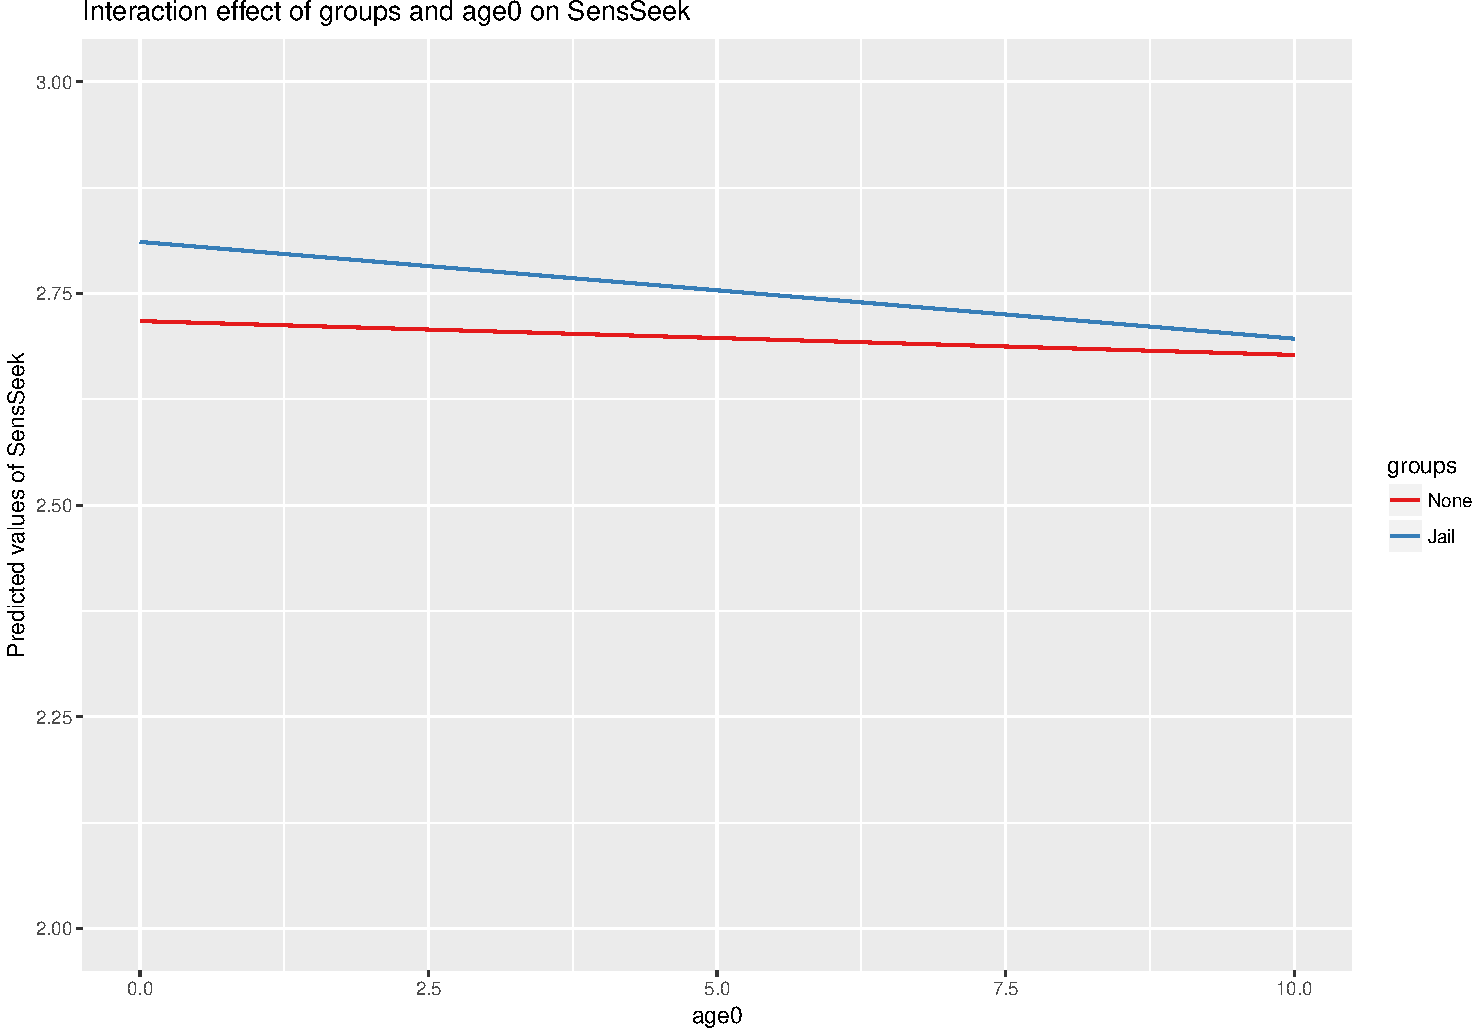
\includegraphics{Conditional_Models_files/figure-beamer/unnamed-chunk-29-1.pdf}

\end{frame}

\begin{frame}[fragile]{Side Note: Plotting Simple Effects (Continuous)}

\small

\begin{Shaded}
\begin{Highlighting}[]
\KeywordTok{sjp.int}\NormalTok{(mod1b, }\DataTypeTok{type =} \StringTok{"eff"}\NormalTok{, }\DataTypeTok{p.kr =} \NormalTok{F, }\DataTypeTok{swap.pred =} \NormalTok{T, }\DataTypeTok{mdrt.values =} \StringTok{"meansd"}\NormalTok{)}
\end{Highlighting}
\end{Shaded}

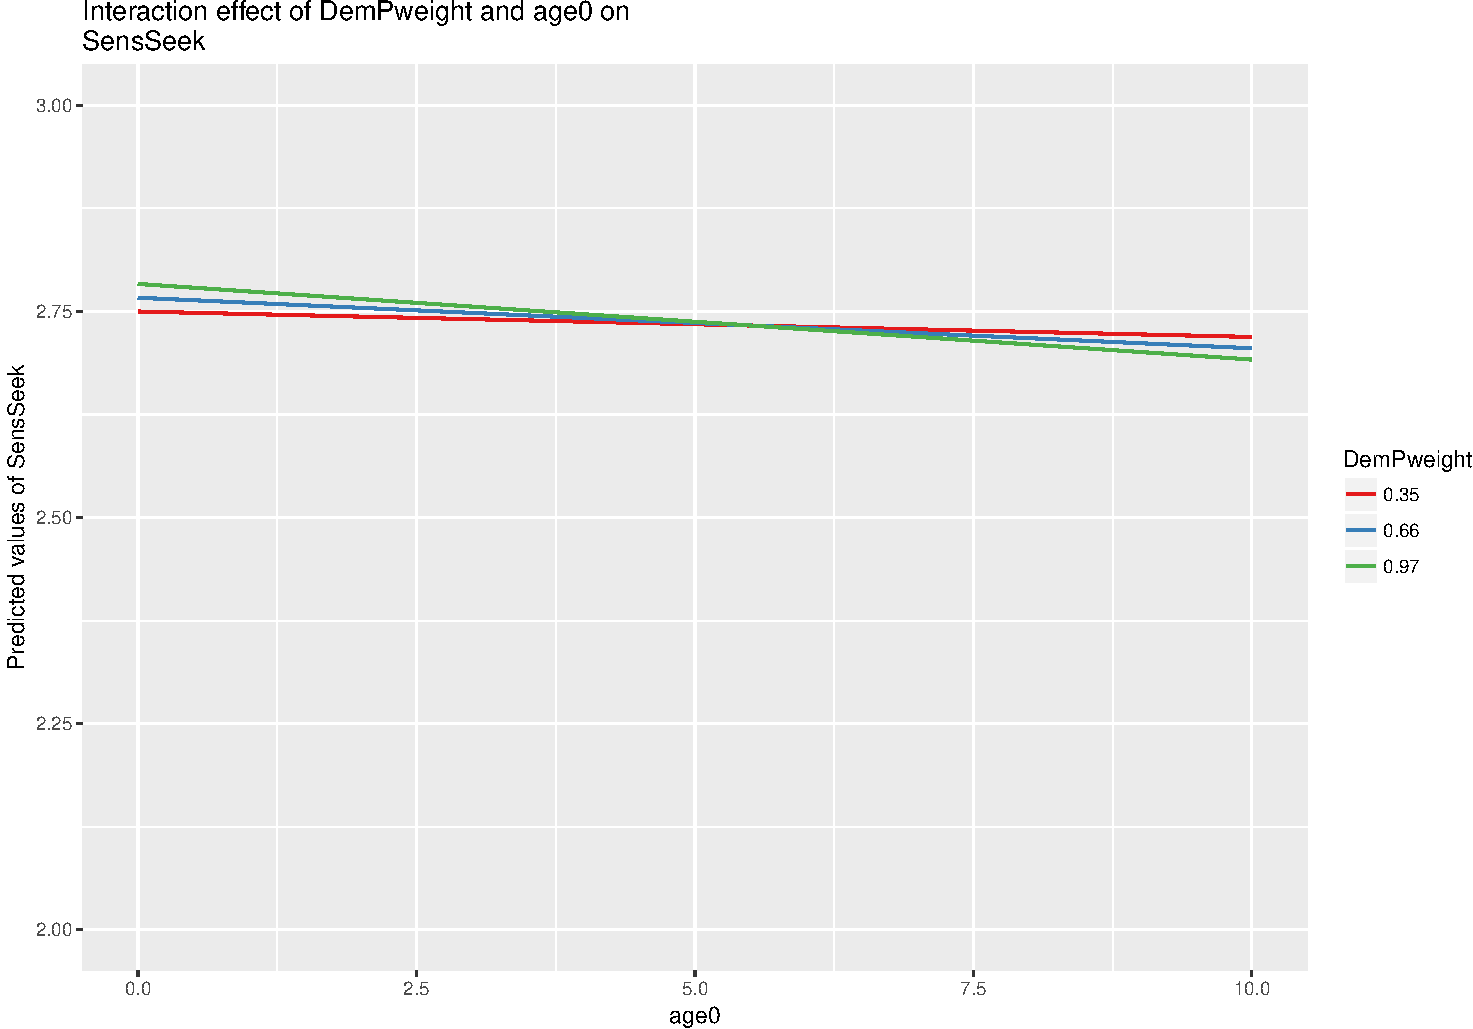
\includegraphics{Conditional_Models_files/figure-beamer/unnamed-chunk-31-1.pdf}

\normalsize  

\end{frame}

\begin{frame}[fragile]{Side Note: Comparisons with \texttt{lsmeans}}

\footnotesize

\begin{Shaded}
\begin{Highlighting}[]
\CommentTok{# create a reference grid}
\NormalTok{ref.grid2g <-}\StringTok{ }\KeywordTok{ref.grid}\NormalTok{(mod2g)}
\CommentTok{# create the lsmeans object}
\NormalTok{lsgroups   <-}\StringTok{ }\KeywordTok{lsmeans}\NormalTok{(ref.grid2g, }\StringTok{"groups"}\NormalTok{)}
\CommentTok{# compact letter display}
\KeywordTok{cld}\NormalTok{(lsgroups, }\DataTypeTok{alpha =} \NormalTok{.}\DecValTok{10}\NormalTok{)}
\CommentTok{# plot}
\KeywordTok{plot}\NormalTok{(lsgroups)}
\CommentTok{# contrasts of the ref.grid object}
\KeywordTok{contrast}\NormalTok{(ref.grid2g, }\DataTypeTok{method =} \StringTok{"eff"}\NormalTok{)}
\CommentTok{# comparisons}
\NormalTok{groups.sum <-}\StringTok{ }\KeywordTok{summary}\NormalTok{(lsgroups, }\DataTypeTok{infer =} \KeywordTok{c}\NormalTok{(}\OtherTok{TRUE}\NormalTok{,}\OtherTok{TRUE}\NormalTok{), }
                      \DataTypeTok{level =} \NormalTok{.}\DecValTok{90}\NormalTok{, }\DataTypeTok{adjust =} \StringTok{"bon"}\NormalTok{, }\DataTypeTok{by =} \StringTok{"groups"}\NormalTok{)}
\end{Highlighting}
\end{Shaded}

\end{frame}

\begin{frame}[fragile]

\begin{Shaded}
\begin{Highlighting}[]
\CommentTok{# create a reference grid}
\NormalTok{(ref.grid2g <-}\StringTok{ }\KeywordTok{ref.grid}\NormalTok{(mod2g))}
\end{Highlighting}
\end{Shaded}

\begin{verbatim}
## 'ref.grid' object with variables:
##     age0 = 3.9123
##     groups = None, Jail
\end{verbatim}

\end{frame}

\begin{frame}[fragile]

\begin{Shaded}
\begin{Highlighting}[]
\CommentTok{# create the lsmeans object}
\NormalTok{(lsgroups   <-}\StringTok{ }\KeywordTok{lsmeans}\NormalTok{(ref.grid2g, }\StringTok{"groups"}\NormalTok{))}
\end{Highlighting}
\end{Shaded}

\begin{verbatim}
##  groups   lsmean         SE     df lower.CL upper.CL
##  None   2.701777 0.02855972 701.42 2.645704 2.757850
##  Jail   2.766199 0.02480113 676.80 2.717505 2.814892
## 
## Degrees-of-freedom method: satterthwaite 
## Confidence level used: 0.95
\end{verbatim}

\end{frame}

\begin{frame}[fragile]

\begin{Shaded}
\begin{Highlighting}[]
\CommentTok{# compact letter display}
\KeywordTok{cld}\NormalTok{(lsgroups, }\DataTypeTok{alpha =} \NormalTok{.}\DecValTok{10}\NormalTok{)}
\end{Highlighting}
\end{Shaded}

\begin{verbatim}
##  groups   lsmean         SE     df lower.CL upper.CL .group
##  None   2.701777 0.02855972 701.42 2.645704 2.757850  1    
##  Jail   2.766199 0.02480113 676.80 2.717505 2.814892   2   
## 
## Degrees-of-freedom method: satterthwaite 
## Confidence level used: 0.95 
## significance level used: alpha = 0.1
\end{verbatim}

\end{frame}

\begin{frame}[fragile]

\begin{Shaded}
\begin{Highlighting}[]
\CommentTok{# plot}
\KeywordTok{plot}\NormalTok{(lsgroups)}
\end{Highlighting}
\end{Shaded}

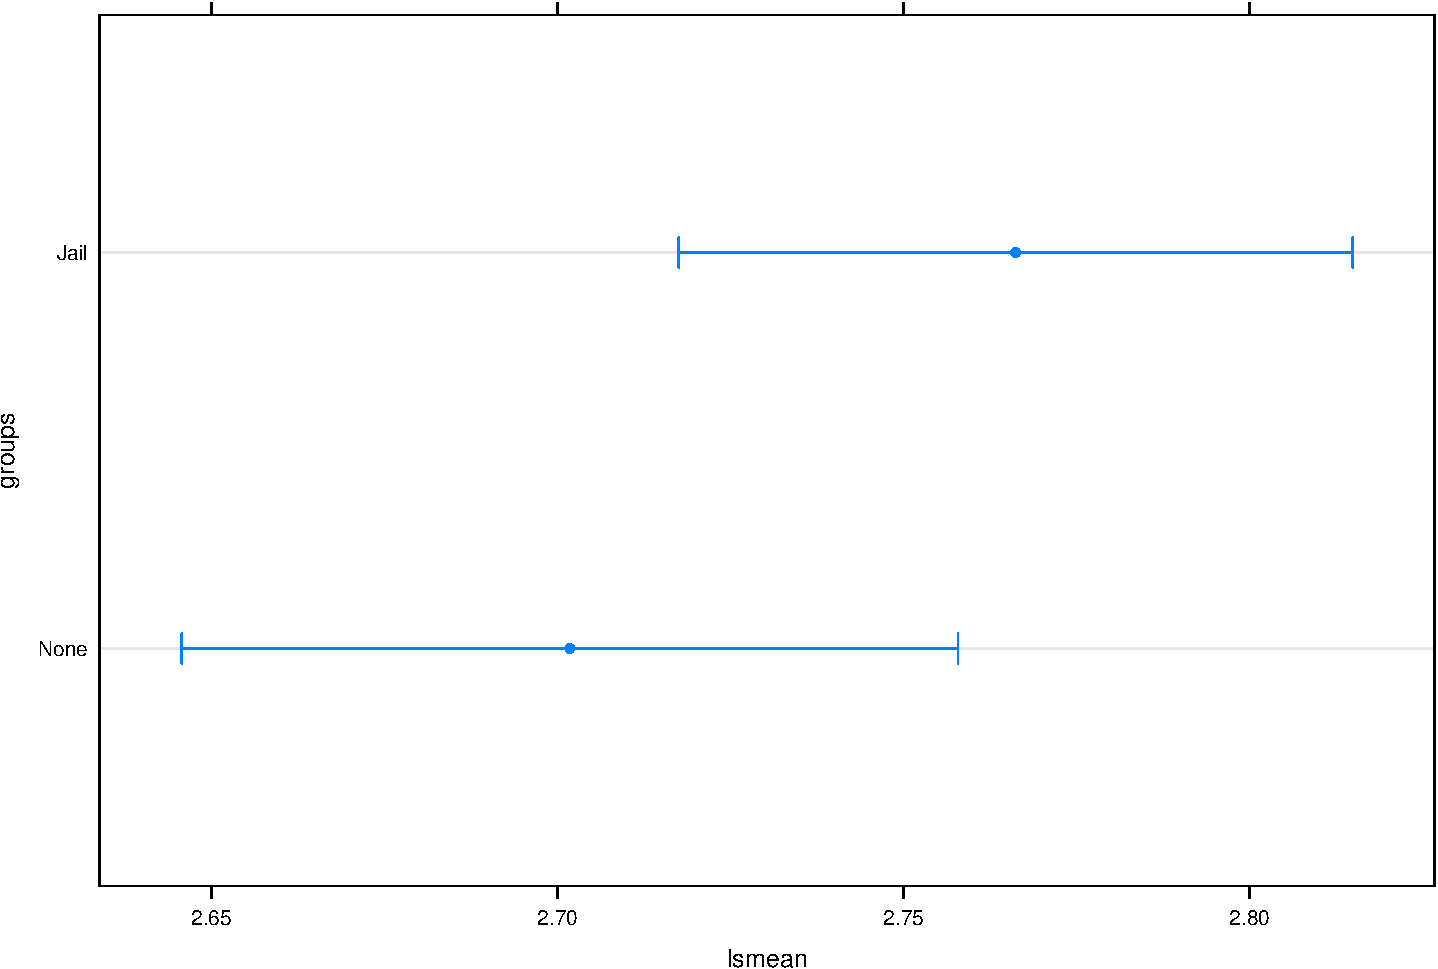
\includegraphics{Conditional_Models_files/figure-beamer/unnamed-chunk-37-1.pdf}

\end{frame}

\begin{frame}[fragile]

\begin{Shaded}
\begin{Highlighting}[]
\CommentTok{# contrasts of the ref.grid object}
\KeywordTok{contrast}\NormalTok{(ref.grid2g, }\DataTypeTok{method =} \StringTok{"eff"}\NormalTok{)}
\end{Highlighting}
\end{Shaded}

\begin{verbatim}
##  contrast                        estimate         SE     df t.ratio
##  3.91226954863318,None effect -0.03221079 0.01891265 690.74  -1.703
##  3.91226954863318,Jail effect  0.03221079 0.01891265 690.74   1.703
##  p.value
##   0.0890
##   0.0890
## 
## P value adjustment: fdr method for 2 tests
\end{verbatim}

\end{frame}

\begin{frame}[fragile]

\begin{Shaded}
\begin{Highlighting}[]
\CommentTok{# comparisons}
\NormalTok{(groups.sum <-}\StringTok{ }\KeywordTok{summary}\NormalTok{(lsgroups, }\DataTypeTok{infer =} \KeywordTok{c}\NormalTok{(}\OtherTok{TRUE}\NormalTok{,}\OtherTok{TRUE}\NormalTok{), }
          \DataTypeTok{level =} \NormalTok{.}\DecValTok{90}\NormalTok{, }\DataTypeTok{adjust =} \StringTok{"bon"}\NormalTok{, }\DataTypeTok{by =} \StringTok{"groups"}\NormalTok{))}
\end{Highlighting}
\end{Shaded}

\begin{verbatim}
## groups = None:
##    lsmean         SE     df lower.CL upper.CL t.ratio p.value
##  2.701777 0.02855972 701.42 2.654739 2.748816  94.601  <.0001
## 
## groups = Jail:
##    lsmean         SE     df lower.CL upper.CL t.ratio p.value
##  2.766199 0.02480113 676.80 2.725351 2.807047 111.535  <.0001
## 
## Degrees-of-freedom method: satterthwaite 
## Confidence level used: 0.9
\end{verbatim}

\end{frame}

\begin{frame}{Time Invariant Predictors: Example - 3 level group}

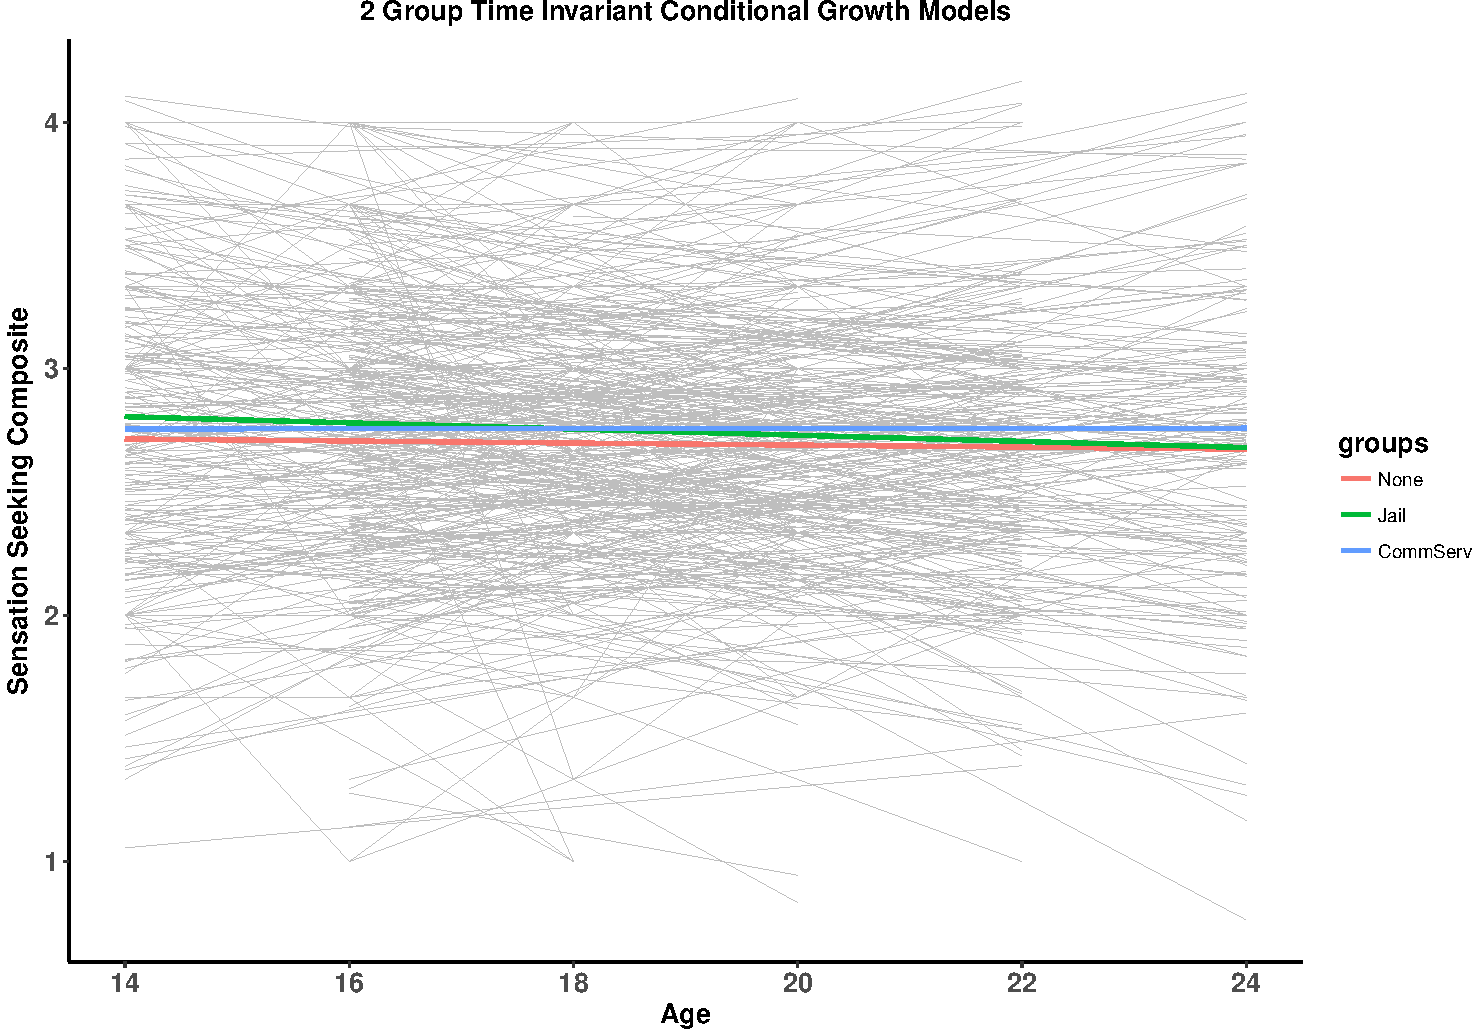
\includegraphics{Conditional_Models_files/figure-beamer/unnamed-chunk-40-1.pdf}

\end{frame}

\begin{frame}{Time Invariant Predictors: Example - 3 level group}

\begin{itemize}
  \item \textbf{Level 1:} $Y_{ij} = \beta_{0j} + \beta_{1j}*age0_{ij} + \varepsilon{ij}$
  \item \textbf{Level 2:} 
    \begin{itemize} 
      \item $\beta_{0j} = \gamma_{00} + \gamma_{01}*D1 + \gamma_{02}*D2 + U_{0j}$
      \item $\beta_{1j} = \gamma_{10} + \gamma_{11}*D1 + \gamma_{12}*D2 + U_{1j}$
    \end{itemize}
\end{itemize}

\begin{longtable}[]{@{}lll@{}}
\toprule
Variable & D1 & D2\tabularnewline
\midrule
\endhead
Jail & 0 & 0\tabularnewline
None & 1 & 0\tabularnewline
CommServ & 0 & 1\tabularnewline
\bottomrule
\end{longtable}

\end{frame}

\begin{frame}[fragile]{Time Invariant Predictors: Example - 3 level
group}

\small

\begin{Shaded}
\begin{Highlighting}[]
\NormalTok{mod3g <-}\StringTok{ }\KeywordTok{lmer}\NormalTok{(SensSeek ~}\StringTok{ }\NormalTok{age0 +}\StringTok{ }\NormalTok{groups +}\StringTok{ }\NormalTok{age0*groups +}\StringTok{ }
\StringTok{                }\NormalTok{(age0|PROC_CID), }\DataTypeTok{data =} \NormalTok{sample_dat)}
\KeywordTok{summary}\NormalTok{(mod3g)}
\end{Highlighting}
\end{Shaded}

\tiny

\begin{verbatim}
## Linear mixed model fit by REML ['lmerMod']
## Formula: SensSeek ~ age0 + groups + age0 * groups + (age0 | PROC_CID)
##    Data: sample_dat
## 
## REML criterion at convergence: 3418.7
## 
## Scaled residuals: 
##     Min      1Q  Median      3Q     Max 
## -3.2994 -0.5006  0.0368  0.4533  3.0815 
## 
## Random effects:
##  Groups   Name        Variance  Std.Dev. Corr 
##  PROC_CID (Intercept) 0.1446194 0.38029       
##           age0        0.0008903 0.02984  -0.23
##  Residual             0.1888364 0.43455       
## Number of obs: 2084, groups:  PROC_CID, 924
## 
## Fixed effects:
##                      Estimate Std. Error t value
## (Intercept)          2.717703   0.035554   76.44
## age0                -0.004101   0.006376   -0.64
## groupsJail           0.092594   0.047097    1.97
## groupsCommServ       0.035192   0.053386    0.66
## age0:groupsJail     -0.007181   0.008265   -0.87
## age0:groupsCommServ  0.005939   0.009871    0.60
## 
## Correlation of Fixed Effects:
##             (Intr) age0   grpsJl grpsCS ag0:gJ
## age0        -0.619                            
## groupsJail  -0.755  0.467                     
## gropsCmmSrv -0.666  0.412  0.503              
## age0:grpsJl  0.478 -0.772 -0.618 -0.318       
## ag0:grpsCmS  0.400 -0.646 -0.302 -0.612  0.498
\end{verbatim}

\normalsize

\end{frame}

\section{Time Varying Predictors}\label{time-varying-predictors}

\begin{frame}{Time Varying Predictors: Continuous}

Next, we'll add in a time-varying predictor. Maybe it's not that our
participants sensation seeking is moderated by early life experiences of
jail or court-ordered community service. Instead, their sensation
seeking is moderated by depression.\\
How does this look?

\begin{itemize}
  \item \textbf{Level 1:} $Y_{ij} = \beta_{0j} + \beta_{1j}*time + \beta_{2j}*CESD + \varepsilon{ij}$
  \item \textbf{Level 2:} 
    \begin{itemize} 
      \item $\beta_{0j} = \gamma_{00} + \gamma_{01} + U_{0j}$
      \item $\beta_{1j} = \gamma_{10} + U_{1j}$
      \item $\beta_{2j} = \gamma_{20}$
    \end{itemize}
\end{itemize}

\end{frame}

\begin{frame}{Time Varying Predictors: Continuous}

\begin{block}{To Interaction or Not - That Is the Question}

\begin{itemize}
  \item \textbf{Level 1:} $Y_{ij} = \beta_{0j} + \beta_{1j}*age0 + \beta_{2j}*CESD + \varepsilon{ij}$
  \item \textbf{Level 2:} 
    \begin{itemize} 
      \item $\beta_{0j} = \gamma_{00} + \gamma_{01} + U_{0j}$
      \item $\beta_{1j} = \gamma_{10} + U_{1j}$
      \item $\beta_{2j} = \gamma_{20}$
    \end{itemize}
\end{itemize}

\[Y_{ij} =  \gamma_{00} + \gamma_{01} + U_{0j} + (\gamma_{10} + U_{1j})*age0 + \gamma_{20}*CESD\]

\end{block}

\end{frame}

\begin{frame}[fragile]{Time Varying Predictors: Continuous}

\small

\begin{Shaded}
\begin{Highlighting}[]
\NormalTok{modTV1 <-}\StringTok{ }\KeywordTok{lmer}\NormalTok{(SensSeek ~}\StringTok{ }\NormalTok{age0 +}\StringTok{ }\NormalTok{CESD +}\StringTok{ }\NormalTok{(age0|PROC_CID), }\DataTypeTok{data =} \NormalTok{sample_dat)}
\end{Highlighting}
\end{Shaded}

\end{frame}

\begin{frame}[fragile]

\tiny

\begin{Shaded}
\begin{Highlighting}[]
\KeywordTok{summary}\NormalTok{(modTV1)}
\end{Highlighting}
\end{Shaded}

\begin{verbatim}
## Linear mixed model fit by REML ['lmerMod']
## Formula: SensSeek ~ age0 + CESD + (age0 | PROC_CID)
##    Data: sample_dat
## 
## REML criterion at convergence: 3391.9
## 
## Scaled residuals: 
##     Min      1Q  Median      3Q     Max 
## -3.4390 -0.5035  0.0363  0.4423  3.1508 
## 
## Random effects:
##  Groups   Name        Variance  Std.Dev. Corr 
##  PROC_CID (Intercept) 0.1412389 0.37582       
##           age0        0.0008117 0.02849  -0.21
##  Residual             0.1892164 0.43499       
## Number of obs: 2084, groups:  PROC_CID, 924
## 
## Fixed effects:
##              Estimate Std. Error t value
## (Intercept)  2.710845   0.025121  107.91
## age0        -0.006475   0.003553   -1.82
## CESD         0.078617   0.021519    3.65
## 
## Correlation of Fixed Effects:
##      (Intr) age0  
## age0 -0.467       
## CESD -0.604 -0.036
\end{verbatim}

\normalsize

\end{frame}

\begin{frame}{Time Varying Predictors: Categorical}

Next, we'll add in a time-varying predictor. Maybe it's not that our
participants sensation seeking is moderated by early life experiences of
jail or court-ordered community service. Instead, their sensation
seeking is moderated by depression.\\
How does this look?

\begin{itemize}
  \item \textbf{Level 1:} $Y_{ij} = \beta_{0j} + \beta_{1j}*time + \beta_{2j}*depressed + \varepsilon{ij}$
  \item \textbf{Level 2:} 
    \begin{itemize} 
      \item $\beta_{0j} = \gamma_{00} + \gamma_{01} + U_{0j}$
      \item $\beta_{1j} = \gamma_{10} + U_{1j}$
      \item $\beta_{2j} = \gamma_{20}$
    \end{itemize}
\end{itemize}

\end{frame}

\begin{frame}[fragile]{Time Varying Predictors: Categorical}

\small

\begin{Shaded}
\begin{Highlighting}[]
\CommentTok{# creating a dummy variable for time varying categorical depression}
\NormalTok{sample_dat <-}\StringTok{ }\NormalTok{sample_dat %>%}
\StringTok{  }\KeywordTok{mutate}\NormalTok{(}\DataTypeTok{depressed =} 
           \KeywordTok{factor}\NormalTok{(}\KeywordTok{ifelse}\NormalTok{(CESD <=}\StringTok{ }\FloatTok{1.5}\NormalTok{, }\DecValTok{0}\NormalTok{, }\DecValTok{1}\NormalTok{), }\DataTypeTok{levels =} \KeywordTok{c}\NormalTok{(}\DecValTok{0}\NormalTok{,}\DecValTok{1}\NormalTok{), }
                  \DataTypeTok{labels =} \KeywordTok{c}\NormalTok{(}\StringTok{"Depressed"}\NormalTok{, }\StringTok{"Not Depressed"}\NormalTok{)))}
\NormalTok{modTV2 <-}\StringTok{ }\KeywordTok{lmer}\NormalTok{(SensSeek ~}\StringTok{ }\NormalTok{age0 +}\StringTok{ }\NormalTok{depressed +}\StringTok{ }\NormalTok{(age0|PROC_CID), }
               \DataTypeTok{data =} \NormalTok{sample_dat)}
\KeywordTok{summary}\NormalTok{(modTV2)}
\end{Highlighting}
\end{Shaded}

\end{frame}

\begin{frame}[fragile]

\tiny

\begin{verbatim}
## Linear mixed model fit by REML ['lmerMod']
## Formula: SensSeek ~ age0 + depressed + (age0 | PROC_CID)
##    Data: sample_dat
## 
## REML criterion at convergence: 3401
## 
## Scaled residuals: 
##     Min      1Q  Median      3Q     Max 
## -3.3686 -0.5094  0.0363  0.4522  3.1406 
## 
## Random effects:
##  Groups   Name        Variance  Std.Dev. Corr 
##  PROC_CID (Intercept) 0.1427349 0.37780       
##           age0        0.0008415 0.02901  -0.21
##  Residual             0.1895332 0.43535       
## Number of obs: 2084, groups:  PROC_CID, 924
## 
## Fixed effects:
##                         Estimate Std. Error t value
## (Intercept)             2.760189   0.020388  135.38
## age0                   -0.006154   0.003564   -1.73
## depressedNot Depressed  0.068617   0.039992    1.72
## 
## Correlation of Fixed Effects:
##             (Intr) age0  
## age0        -0.599       
## dprssdNtDpr -0.174 -0.024
\end{verbatim}

\normalsize

\end{frame}

\section{confidence intervals and effect
size}\label{confidence-intervals-and-effect-size}

\section{fitted / predicted values}\label{fitted-predicted-values}

\section{Other Things}\label{other-things}

\section{autoregressive models, autoregressive
errors}\label{autoregressive-models-autoregressive-errors}

\section{cohen's d - changing intercept with 0 at last time
point}\label{cohens-d---changing-intercept-with-0-at-last-time-point}

\end{document}
